%导言区
\documentclass[12pt]{ctexart}
\title{\vspace{-1.5cm} \zihao{3} \heiti 无人机纯方位无源定位模型}
\date{}

%********************包的引用****************%
% 页面设置
\usepackage{fancyhdr}        % 页脚页眉
\usepackage{lastpage}        % 获取总共的页数
\usepackage{geometry}        % 设置页边距
% 修改摘要
\usepackage{abstract}
% 数学环境
\usepackage{amsmath}
\usepackage{amssymb}
% 矩阵斜省略号iddots
\usepackage{mathdots}
% 插入图片
\usepackage{graphicx} 		% 插入图片的宏包(can't graphics)
\usepackage{float} 			% 设置图片浮动位置的宏包
\graphicspath{{./figure/}}  % 搜索路径
\usepackage{subfigure} 		% 多图排版
% 三线表
\usepackage{booktabs}
% 间距宏包
\usepackage{setspace}
% 文字加颜色
\usepackage{color}
\usepackage{xcolor}
% 插入代码宏包
\usepackage{listings}
\usepackage{appendix} % 附录
%
\usepackage{multirow}

%*******************全文格式设置********************%

% 设置纸张为A4,上下边距为3.2、2.8cm,左右边距为2.5cm 
\geometry{a4paper,left=2.5cm,right=2.5cm,top=2.5cm,bottom=2.5cm}

% 各级标题格式的设置
\setcounter{tocdepth}{4}     % 设置目录显示的深度为4
\setcounter{secnumdepth}{4}  % 设置章节显示的深度为4
\ctexset{
	% 黑体小三,居中对齐,段前段后30pt
	section={
		format=\zihao{-3} \heiti \centering,
		name = {,、},
		number = \chinese{section},
		aftername=\hspace{0pt},
		beforeskip=30pt,
		afterskip=30pt
	},
	subsection={
		format = \zihao{-3} \heiti \raggedright,
		beforeskip=18pt,
		afterskip=12pt
	},
	subsubsection={
		format=\fontsize{13pt}{20pt} \heiti \raggedright,
		beforeskip=12pt,
		afterskip=12pt,
	},
	paragraph={
		format=\zihao{-4} \songti \raggedright,
		beforeskip=6pt,
		afterskip=6pt,
	}
}

% 摘要格式设置
\setlength{\abstitleskip}{-1em} % 摘要标题和内容的间距
\setlength{\absleftindent}{6pt}
\setlength{\absrightindent}{6pt}
\renewcommand{\abstractnamefont}{\zihao{4} \centering \heiti}
\renewcommand{\abstracttextfont}{\zihao{-4} \songti}

% 附录格式设置
\lstset{
	numbers=left, % 行号显示在左边
	numberstyle=\tiny, % 行号字体为tiny
	basicstyle=\ttfamily, % 设置字体族
	breaklines=true, % 自动换行
	frame=shadowbox, % 边框
	% 设置关键词
	keywordstyle=\color{blue!70},
	morekeywords={}, % 设置更多的关键字,用逗号分隔
	% 设置注释样式(斜体)
	commentstyle=\itshape\color{red!50!green!50!blue!50},
	% 代码块边框颜色
	rulesepcolor=\color{red!20!green!20!blue!20},
	% 左右页边距
	xleftmargin=1em,xrightmargin=1em,
	% 上页边距
	aboveskip=-1em,
	% 背景颜色
	backgroundcolor=\color{white}
} 

% 设置页码
\pagestyle{fancy}     % 使用fancy风格
\fancyhf{}            % 清除所有的页眉页脚
\renewcommand\headrulewidth{0pt}   % 去除页眉横线
\fancyfoot[C]{\thepage}   % 页码

% 全文设置1.5倍间距
\setlength{\baselineskip}{20pt}     
% \renewcommand{\baselinestretch}{1.5}  % 全文设置1.5倍间距

% 参考文献样式
\bibliographystyle{plain}
% 定义参考文献的数字为右上角的命令:\supercite
% 1个参数,#1传参,\textsuperscript文本环境下的上标
\newcommand\supercite[1]{\textsuperscript{\cite{#1}}}


%******************正文区******************%
\begin{document}
\begin{spacing}{1.5}
	
\maketitle	% 设置标题
\setcounter{page}{1}  % 从此页开始编页码
% \thispagestyle{empty} % 不计此页页数
% \tableofcontents      % 显示目录

\vspace{-6.5em}
% \vspace*{-2.5cm} % 向上缩进
%**********************摘要*******************%

\begin{abstract}
	\setlength
	无人机编队飞行的用途相当广泛,它不仅给人以视觉上的享受,还可用于军事,实现密集突防。本文主要研究纯方位无源定位情形下的无人机定位问题,建立了接收信号无人机的定位模型,利用几何分析法、优化模型进行求解,并对模型进行验证。
	
	{\heiti 针对问题1.1:}无人机的定位问题。定位模型建立过程如下:首先,基于10架无人机各自的位置信息和编号信息,以及接收信号无人机所收到的方位角度信息,由夹角余弦定理建立利用定位三角形的重心确定方程组的解;其次,通过方位角度信息与发射信号无人机编号之间的对应关系,建立6组关联角度和编号的方程,得到6组解,并将所求解与理想解之间最小值的平方和设置为目标函数,从而找到与理想解最近的解;最后,确定定位模型最终解并得出定位模型,利用问题1.3中的数据对模型进行检验,效果良好。
	
	{\heiti 针对问题1.2:}发射源位置位置时无人机的定位问题。由问题1.1知只需要由接收信号确定发射源即可。通过对角度规律的分析,在偏离位置较小的情况下,只需额外添加2架发射信号无人机就可以有效定位。
	
	{\heiti 针对问题1.3:}圆形编队调整位置的方案选择问题。首先,基于2架发射信号无人机的编号已知且位置无偏差的情形,选取两个固定点(FY00、FY01)和一到两个未知点(与理想位置最近的无人机)发射信号;其次,基于定位模型得到的位置和理想位置之间的误差,对位置的调整进行迭代处理;以误差平方和为目标函数建立优化模型,利用$Matlab$求解得出需进行6次调整才能使9架无人机均匀分布于圆周上,最终距离误差在0.01米以内。
	
	{\heiti 针对问题2:}利用锥形编队的几何特征,将15架无人机用6个圆形编队进行覆盖。选取编号是FY03、FY05、FY07、FY08、FY09和FY14的无人机作为6个圆心,依次调整6个圆周上无人机的位置使之能够均匀分布。基于问题1.3求解的方法,对锥形中15架无人机的位置进行调整,设计出锥形编队调整方案的算法。
	
	最后,我们对模型进行了讨论和分析,做出了客观的优缺点评价。\\
	\textbf{关键词:}纯方位无源定位 \quad 定位三角性 \quad 目标优化 \quad 余弦公式
\end{abstract}

\newpage % 新的一页
\section{问题重述}
\subsection{问题背景}
在遂行编队飞行中,无人机有两种类型:一种用于发射信号,另一种用于接收信号。每一架无人机之间通过信号的传递微调方位,即利用纯方位无源定位对无人机的位置进行调整,从而保持编队的队形。其中,被动接收信号的无人机将收到“自身与任何两架发射信号的无人机连线间夹角”的方向信息。编队中每一架无人机都有固定的编号。
\subsection{需要解决的问题}
1架编号为FY00的无人机位于圆心,其余9架编号为FY01~FY09的无人机则均匀分布于某一圆周上,形成圆形编队。飞行中,所有无人机的高度是相同且不变的。

{\heiti 问题1.1:}已知发射信号无人机(位于圆心的FY00和编队中另外2架)的编号且其位置无偏差,建立被动接收信号无人机(位置略有偏差)的定位模型。

{\heiti 问题1.2:}接收信号无人机位置略有偏差,假设发射信号无人机(FY00、FY01和编队中若干编号未知的)位置无偏差,求出为有效定位无人机所需添加的发射信号无人机的数量。

{\heiti  问题1.3:} 要求形成圆形编队,圆心有1架无人机,半径为$100m$的圆周上均匀分布着另外9架无人机。根据表1的数据,已知部分无人机的初始位置略有偏差,给出无人机位置具体的调整方案(不考虑每次调整的时间),使9架无人机最后在某个圆周上均匀分布。每次调整中,最多有4架发射信号的无人机(FY00和圆周上至多3架),其余均为接收方向信息的无人机。

{\heiti 问题2:}应用纯方位无源定位的方法,设计无人机位置的调整方案,使得直线上相邻两架无人机的距离是相等的,即形成锥形编队。

\section{问题分析}
问题1为无人机在飞行形成圆形编队过程中的定位与位置调整方案的选择问题。其中,问题1.1、问题1.2均为定位问题,问题1.3为方案选择问题。问题2为无人机集群在形成锥形编队过程中的位置调整方案的选择问题。
\subsection{问题1.1的分析}
对于问题1.1,3架发射信号无人机的编号已知且位置无偏差,因此被动接收信号的无人机所收到的方位信息即为实际的位置信息。由于接收信号无人机的位置有偏差,考虑到其将收到3个夹角的角度信息且夹角与3架已知编号无人机的对应关系是未知的,因此本文先通过几何关系分析并建立夹角角度与已知编号无人机位置的关系式,再从有限解中找到与被动定位无人机的理想位置最近的解,以期建立三站纯方位无源定位模型。
\subsection{问题1.2的分析}
对于问题1.2,接收信号无人机的位置稍有偏差且其编号是否已知并未明确,因此将其分成编号已知和编号未知两种情况分析。此问采用角度大小与相对位置关系对未知的编号进行确定,巧妙地将问题转化为“使编号确定的最少的无人机数目”这一目标求解问题。根据圆周角等于其所对圆心角的一半,分析得出圆周上两架无人机与接收源所形成夹角的角度为20n°(n为整数),以及根据已确定编号无人机的数量得到各个夹角的角度关系式,尝试建立与发射信号无人机数量和夹角角度相关的有效定位模型。
\subsection{问题1.3的分析}
问题1.3需要将初始位置有偏差的无人机调整到理想位置上,考虑到编号为FY00、FY01的无人机的初始位置是无偏差的,且发射信号无人机的数量是有限制的,因此该问选取“两个定点、一个或两个未知点”发射信号,对接收信号的无人机进行定位并给出调整方案。其次,考虑实际定位与理想位置之间的误差,此问需通过迭代多次调整位置,以建立定位模型和设计调整方案的选取算法。
\subsection{问题2的分析}
问题2是问题1.3的拓展。此问基于问题1.3的圆形编队调整位置的算法,将分别以FY05、FY08、FY09为圆心,靠近圆心最近的6架无人机分别均匀分布于3个圆周上,依次调整3个圆周上的无人机位置,建立定位模型和设计调整方案的选取算法。

\section{模型的假设}
1.假设接收信号无人机的编号和理想位置已知;

2.假设无人机之间传递的所有信息均是准确无误的;

3.所有无人机在飞行过程中的高度是相同且不变的;

4.调整无人机的方位时,不考虑每次调整的时间。

\section{符号说明}
\begin{center}	
\begin{tabular}{cc}		
\toprule[1.5pt]		
\makebox[0.3\textwidth][c]{符号}	&  \makebox[0.4\textwidth][c]{意义}\\
\midrule[0.5pt]		
$ i,j(i,j=0,1,2,...,9) $				& 发射信号无人机的编号 \\
$ k(k=0,1,2,...,9) $					& 接收信号无人机的编号 \\
$ \alpha_{ij}(i,j=0,1,2,...,9) $		& FY0i与FY0j发射信号之间的夹角 \\
$ (x_{k},y_{k})(k=0,1,2,...,9) $			& FY0k的坐标 \\
$ (x_{m}^{(*)},y_{m}^{(*)})(k=0,1,2,...,9) $	& 编号为$m$的无人机的理想坐标 \\
$ (x_{m}^{(q)},y_{m}^{(q)})(m=3,4,5,...,9) $	& 编号为$m$的无人机接收信号时定位到的坐标 \\
$ (x_{m}^{(k)},y_{m}^{(k)})(m=3,4,5,...,9) $	& 第$k$次迭代求出的编号为$m$的无人机的坐标 \\
$ d_m $				& 编号为$m$的无人机定位位置与实际位置间的距离 \\
$ d $				& 编号为$m$的无人机定位位置与实际位置间的平均距离 \\
$ d_{m}^{k} $		& 第$k$次迭代求出的编号为$m$的无人机与理想位置的距离 \\
$ d^{k} $			& 第$k$次迭代求出的所有无人机与理想位置的最大距离 \\
$ E^2 $				& 能够容忍的最大距离平方 \\
\bottomrule[1.5pt]	
\end{tabular}
\end{center}

\section{模型建立、求解与检验}
\subsection{问题1.1的模型建立与求解}
以编号为FY00的无人机所在位置为坐标原点,指向FY01的方向为$x$轴正方向建立坐标系。

假设发射源无人机编号为$0,i,j$,接收信号无人机编号为$k$,其接收到的方位信息为$(\alpha_{1},\alpha_{2},\alpha_{3})$。由于不知道方位信息与发射源编号之间的对应关系,因此共有$A_3^2$种情形。而问题1.1中已知无人机稍有偏差,利用夹角余弦公式计算对应的坐标信息,并对六种结果选取离理想坐标最近的作为定位坐标。
\begin{figure}[H]
	\centering
	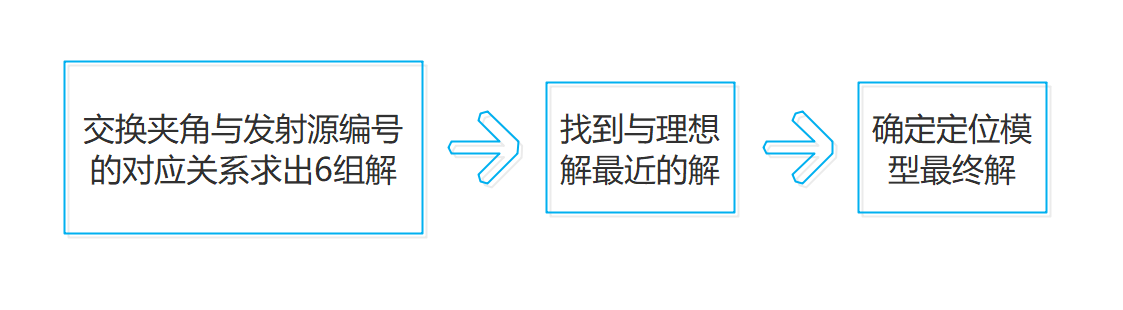
\includegraphics[width=0.8\textwidth]{思路图.png}
	\caption{思路图}
	\label{tu1}
\end{figure}

\subsubsection{信号几何关系分析}
下面我们选择编号为0、$i$、$j$作为信号发射源,选择$k$作为信号接收源进行绘图分析,示意图如下:
\begin{figure}[H]
	\centering
	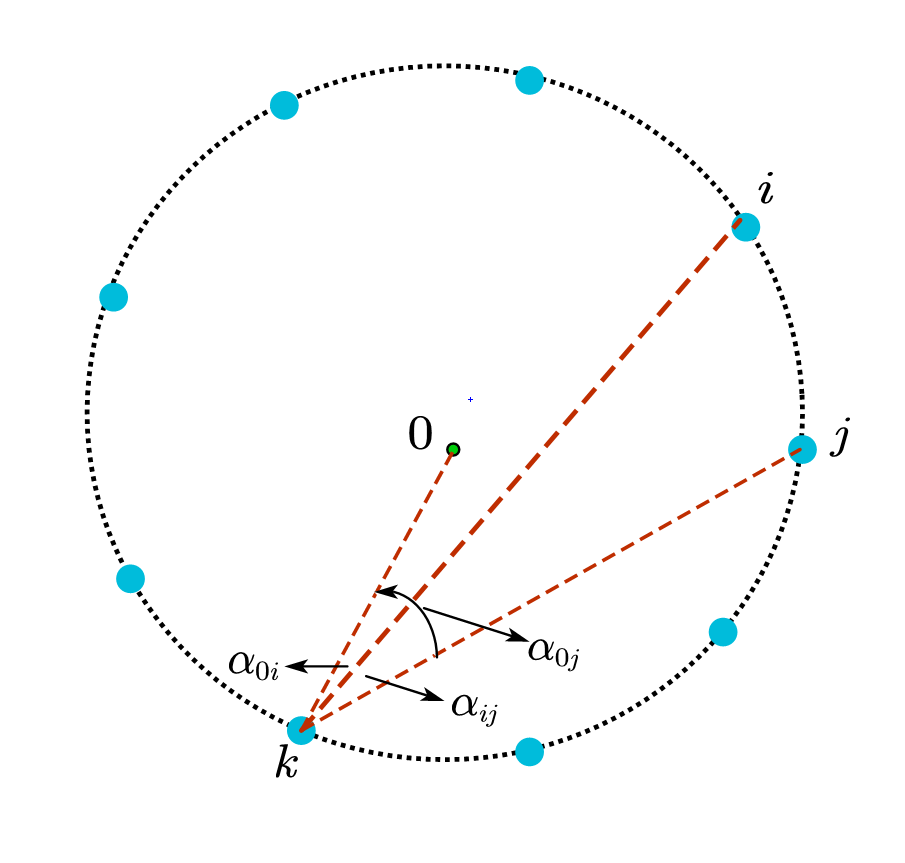
\includegraphics[width=0.8\textwidth]{信号几何关系图.png}
	\caption{信号几何关系图}
	\label{tu2}
\end{figure}
通过分析几何关系,由夹角余弦公式$cos(\vec{m},\vec{n})=\frac{\vec{m}.\vec{n}}{|\vec{m}|.|\vec{n}|}$可得下列关系式:
\begin{equation}
\begin{cases}
	cos(\alpha_{0i})= \frac{(x_0-x)(x_i-x)+(y_0-y)(y_i-y)} {\sqrt{(x_0-x)^2+(y_0-y)^2}\sqrt{(x_i-x)^2+(y_i-y)^2}}\\
	cos(\alpha_{0j})= \frac{(x_0-x)(x_i-x)+(y_0-y)(y_j-y)} {\sqrt{(x_0-x)^2+(y_0-y)^2}\sqrt{(x_j-x)^2+(y_j-y)^2}}\\
	cos(\alpha_{ij})= \frac{(x_i-x)(x_j-x)+(y_i-y)(y_j-y)} {\sqrt{(x_i-x)^2+(y_i-y)^2}\sqrt{(x_j-x)^2+(y_j-y)^2}}
\end{cases}
\label{gs1}
\end{equation}

其中,$\alpha_{0i}$表示编号为0和$i$的无人机发射的信号之间的夹角,$\alpha_{0j}$表示0与$j$对应夹角,$\alpha_{ij}$表示$i$与$j$对应夹角,$(x_0,y_0),(x_i,y_i),(x_j,y_j)$分别表示编号为$0$、$i$、$j$的无人机的坐标。

\subsubsection{编号与夹角对应关系已知情况下方程组的求解}
考虑在编号与夹角对应关系已知的情形下,$\alpha_{0i},\alpha_{0j},\alpha_{ij},(x_0,y_0),(x_i,y_i),(x_j,y_j)$已知,共计三个方程、两个未知量$P(x,y)$。

\textbf{5.1.2.1 解的存在性分析:}

(1)理论上只需要任意两个方程即可解出$P$点坐标,但是由于方程组\ref{gs1}中任意方程均超过一次,可能产生冗余解。由于已知$P$点的理想位置,可以通过解与理想位置的距离排除掉明显不合理的情况。

(2)现在通过三个方程求解$P$点坐标:理想情况下,$P$点坐标满足方程组\ref{gs1},方程组\ref{gs1}解的个数为有限个,一定可以通过求解方程组\ref{gs1}求出$P$点坐标;实际上,由数值误差,每两个方程求出的解(总计三组)可能存在一定的误差,使得求解三个方程无法成功。

\textbf{5.1.2.2 方程组解的处理:}

接收信号无人机收到了三个方向发来的信号,即三条始发于已知编号无人机的射线,每两条射线有一个夹角。

(1)理想情况下,三线交于一点;

(2)存在较小数值误差的情况下,三线交于三点且形成了一个较小的三角性区域,定位坐标大致位于三角性区域内。

使用几何图形说明这一关系,图中最大的蓝色点表示接收信号无人机,红色实线无误差时的情况;蓝色虚线表示有误差时的情况,红色实心点表示有误差时,由三个方程中两个方程求出的解,图中三条射线围成了一个三角形区域$ABC$,可以通过这三个点围成的区域估计出更合理的解。

示意图如下:
\begin{figure}[H]
	\centering
	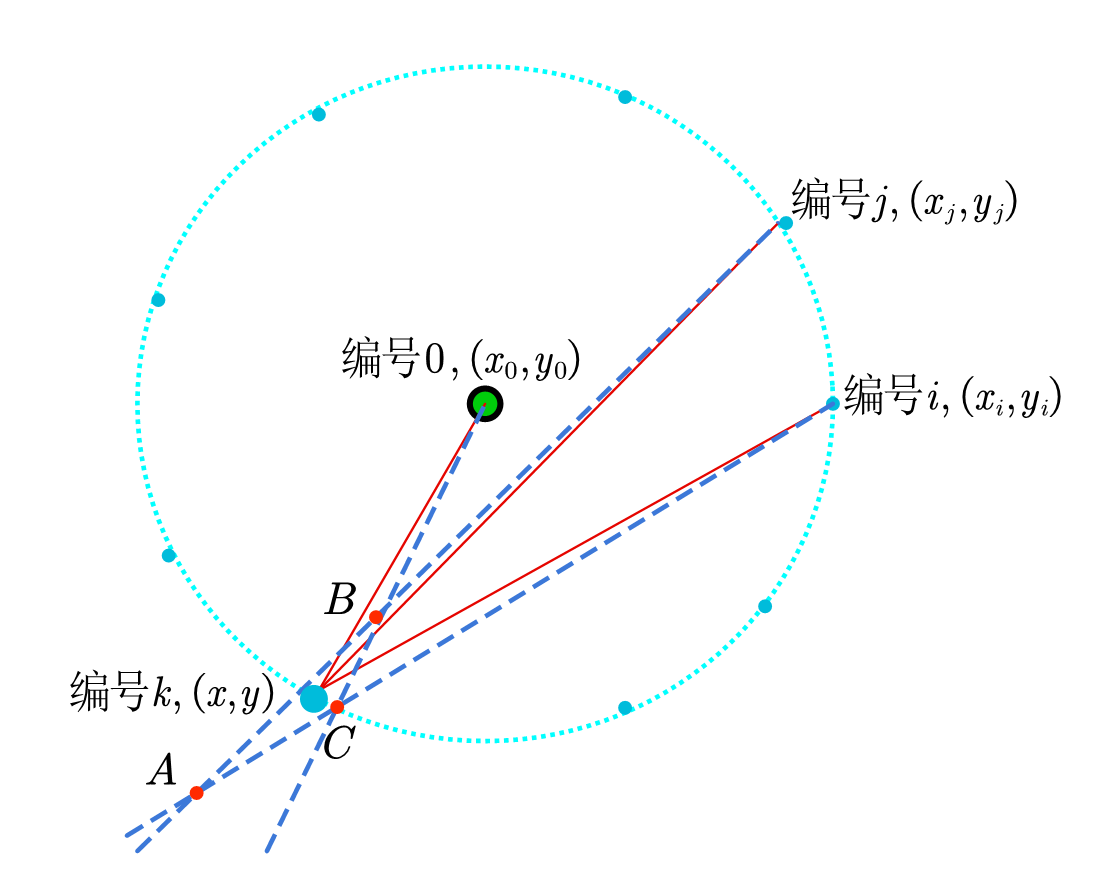
\includegraphics[width=0.8\textwidth]{几何分析法图.png}
	\caption{几何分析法图}
	\label{tu3}
\end{figure}

有偏差时的估计方法:

将三角形$ABC$称为定位三角形\supercite{参考文献1},问题转化为求“定位三角形”的质心。

(1)重心法(计算三角形的重心):
\begin{equation}
	\begin{cases}
		x=\frac{x_A+x_B+x_C}{3}\\
		y=\frac{y_A+y_B+y_C}{3}
	\end{cases}
\end{equation}

(2)内心法(计算三角形的内心):
\begin{equation}
	\begin{cases}
		x=\frac{ax_A+bx_B+cx_C}{a+b+c}\\
		y=\frac{ay_A+by_B+cy_C}{a+b+c}
	\end{cases}
\end{equation}
其中,$a,b,c$为三角形三边的长度,可以通过点$A,B,C$的坐标求出。

从中选择重心法代入模型求解。

\subsubsection{编号与夹角对应关系未知情况下方程组的求解}
已知:$\{\alpha|\alpha=\alpha_{0i},\alpha_{0j},\alpha_{ij}\}=\{\alpha|\alpha=\alpha_{1},\alpha_{2},\alpha_{3}\}$
通过下列任一条件与方程组\ref{gs1}联立求得结果。
\begin{equation}
\begin{cases}
	\alpha_{0i}=\alpha_{1} \\
	\alpha_{0j}=\alpha_{2} \\
	\alpha_{ij}=\alpha_{3} 
\end{cases}
\begin{cases}
	\alpha_{0i}=\alpha_{1} \\
	\alpha_{0j}=\alpha_{3} \\
	\alpha_{ij}=\alpha_{2}  
\end{cases}
\begin{cases}
	\alpha_{0i}=\alpha_{2} \\
	\alpha_{0j}=\alpha_{1} \\
	\alpha_{ij}=\alpha_{3}  
\end{cases}
\begin{cases}
	\alpha_{0i}=\alpha_{2} \\
	\alpha_{0j}=\alpha_{3} \\
	\alpha_{ij}=\alpha_{1}  
\end{cases}
\begin{cases}
	\alpha_{0i}=\alpha_{3} \\
	\alpha_{0j}=\alpha_{1} \\
	\alpha_{ij}=\alpha_{2}  
\end{cases}
\begin{cases}
	\alpha_{0i}=\alpha_{3} \\
	\alpha_{0j}=\alpha_{2} \\
	\alpha_{ij}=\alpha_{1}  
\end{cases}
\label{gs2}
\end{equation}

求得6组解:$(x^{(1)},y^{(1)}),(x^{(2)},y^{(2)}),(x^{(3)},y^{(3)}),(x^{(4)},y^{(4)}),(x^{(5)},y^{(5)}),(x^{(6)},y^{(6)})$,由接收信号的无人机编号可得,对应的理想解为$(x^{(*)},y^{(*)})$。则由

\begin{equation}
Min \quad (x^{(k)}-x^{(*)})^2 + (y^{(k)}-y^{(*)})^2
\end{equation}
$$ s.t.\quad k\in{\{1,2,3,4,5,6\}} $$

可得最终解为:$(x^{(k)},y^{(k)})$。

\subsubsection{方程组求解的一般步骤}
最终求解按照以下规则:

(1)在方程\ref{gs2}中六选一,给定夹角与已知编号一个对应关系;

(2)通过方程组\ref{gs1}中每两个方程得到一个解,若有冗余解,按照与理想解的距离远近排除;

(3)将得到的三个解选取重心法进行平均,得到偏差较小的最优解;

(4)此时得到了一个解$(x^{(1)},y^{(1)})$,重新进行第1步不重复的交换顺序,求出所有基本解$(x^{(1)},y^{(1)})$,$(x^{(2)},y^{(2)})$,$(x^{(3)},y^{(3)})$,$(x^{(4)},y^{(4)})$,$(x^{(5)},y^{(5)})$,$(x^{(6)},y^{(6)})$;

(5)根据与理想解$(x^{(*)},y^{(*)})$的距离求出最终解$(x^{(k)},y^{(k)})$;

(6)定位完成。

求解流程图,如下图\ref{tu12}显示:
\begin{figure}[H]
	\centering
	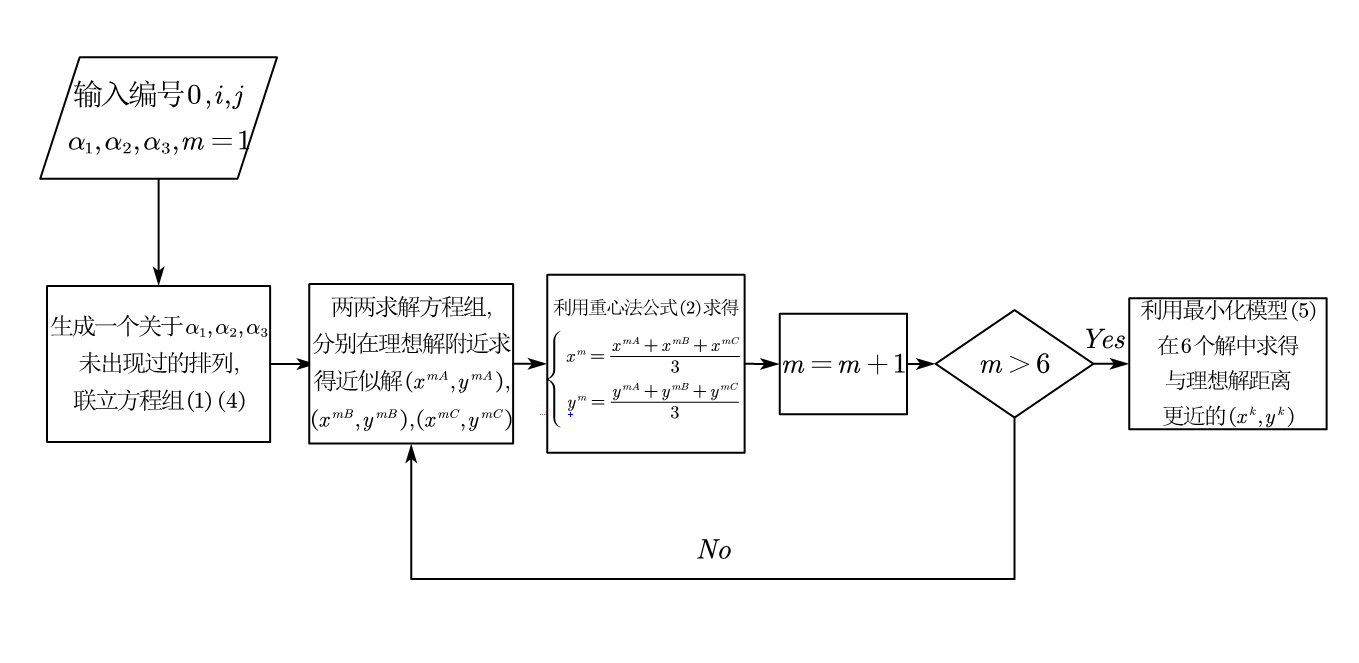
\includegraphics[width=1.0\textwidth]{1.1流程图.png}
	\caption{1.1流程图}
	\label{tu12}
\end{figure}

\subsubsection{模型求解与检验}
\textbf{5.1.5.1 模型误差检验的方法\supercite{参考文献2}:}

距离:
\begin{equation}
	d_m=\sqrt{ (x_{m}^{(k)}-x_{m}^{(q)})^2 + (y_{m}^{(k)}-y_{m}^{(q)})^2 }
\end{equation}

平均距离:
\begin{equation}
	d = \frac{\sqrt{ (x_{m}^{(k)}-x_{m}^{(q)})^2 + (y_{m}^{(k)}-y_{m}^{(q)})^2 }}{7} 
\end{equation}

$x$坐标的相对误差:
\begin{equation}
	e_{m}^{(x)} = |\frac{x_{m}^{(k)}-x_{m}^{(q)}}{x_{m}^{(q)}}|
\end{equation}

$y$坐标的相对误差:
\begin{equation}
	e_{m}^{(y)} = |\frac{y_{m}^{(k)}-y_{m}^{(q)}}{y_{m}^{(q)}}|
\end{equation}

坐标相对误差:
\begin{equation}
	\overline{e_m} = \frac{e_{m}^{(x)}+e_{m}^{(y)}}{2}
\end{equation}

平均坐标相对误差:
\begin{equation}
	\overline{e} = \frac{\sum_{i=3}^{9}\overline{e_i}}{7}
\end{equation}

其中$m=3,4,5,6,7,8,9$,表示接收信号的无人机编号;$x_m^{(q)}$表示编号为$m$的无人机接收信号时定位到的横坐标,$y_m^{(q)}$此时定位到的纵坐标;$x_m^{(k)}$表示编号为$m$的无人机实际的横坐标,$y_m^{(k)}$此时实际的纵坐标。

\textbf{5.1.5.2 下面进行模型的求解和检验:}

选择发射信号的无人机编号为FY00、FY01和FY02验证模型的可行性,自定义满足题目要求的数据加随机小误差,使用建立的模型和$Matlab$函数$vpasolve$,以理想解为初始值,并以发射源到接收源实际的方位信息为输入信息,依次算出FY03、FY04、FY05、FY06、FY07、FY08和FY09的定位坐标,分别计算与实际坐标的距离、$x$坐标的相对误差、$y$坐标的相对误差,并求出平均坐标距离、坐标的平均相对误差,从而绘制误差条形图并检验模型的优劣。

通过对比各点的理想坐标和各点的定位坐标,发现定位坐标十分精确。且如图\ref{tux},FY00、FY01、FY02为发射源模拟求解的坐标与实际坐标的距离条形图及坐标的相对偏差条形图显示:求解模型可解,误差数量级分别在$10^{-13},10^{-14}$,说明精确度很高。

\begin{center}
\begin{table}[H]
	\centering
	\begin{tabular}{cccc}
		\toprule[1.5pt]
		x的理想值        & y的理想值        & x的计算值        & y的计算值        \\ 
		\midrule[1pt]
		19.04420117  & 110.3690102  & 19.04420117  & 110.3690102  \\
		-52.10273289 & 91.16087552  & -52.10273289 & 91.16087552  \\
		-92.00770215 & 33.74289178  & -92.00770215 & 33.74289178  \\
		-105.2722907 & -38.23277145 & -105.2722907 & -38.23277145 \\
		-52.38886564 & -90.99674037 & -52.38886564 & -90.99674037 \\
		17.30380046  & -96.46024305 & 17.30380046  & -96.46024305 \\ 
		\bottomrule[1.5pt]
	\end{tabular}
	\caption{理想坐标与数据坐标}
	\label{b2}
\end{table}
\end{center}

\begin{center}
\begin{table}[H]
	\centering
	\begin{tabular}{cccc}
		\toprule[1.5pt]
		x的相对误差      & y的相对误差      & 坐标相对误差      & 距离          \\ 
		\midrule[1pt]
		4.10412E-15 & 1.28758E-16 & 2.11644E-15 & 7.94411E-14 \\
		8.1824E-16  & 9.35326E-16 & 8.76783E-16 & 9.53293E-14 \\
		3.08906E-16 & 2.10576E-15 & 1.20733E-15 & 7.65278E-14 \\
		2.29485E-15 & 5.2037E-15  & 3.74928E-15 & 3.12962E-13 \\
		5.42514E-16 & 3.12338E-16 & 4.27426E-16 & 4.01944E-14 \\
		9.64976E-15 & 1.17859E-15 & 5.41417E-15 & 2.02005E-13 \\ 
		\bottomrule[1.5pt]
	\end{tabular}
	\caption{模型误差}
	\label{b3}
\end{table}
\end{center}

\begin{figure}[H]
	\centering
	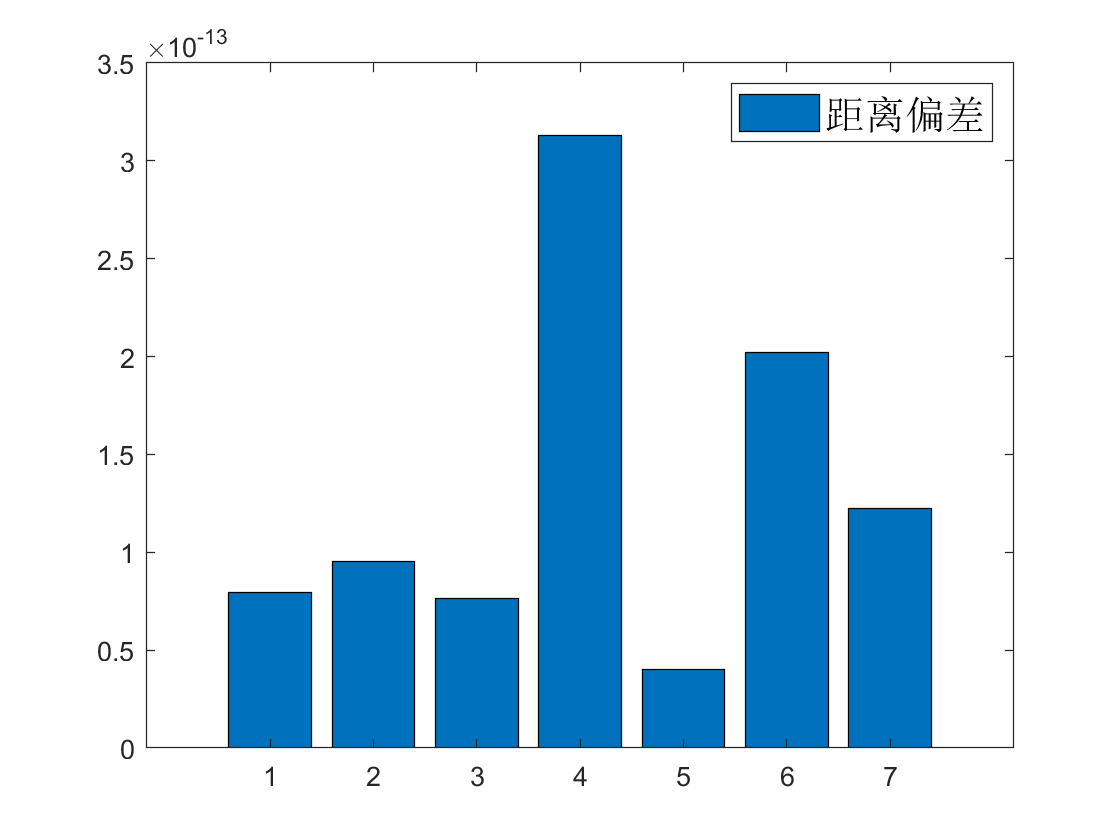
\includegraphics[width=0.7\textwidth]{dd.png}
	\caption{距离条形图}
	\label{tu4}
\end{figure}

\begin{figure}[H]
	\centering
	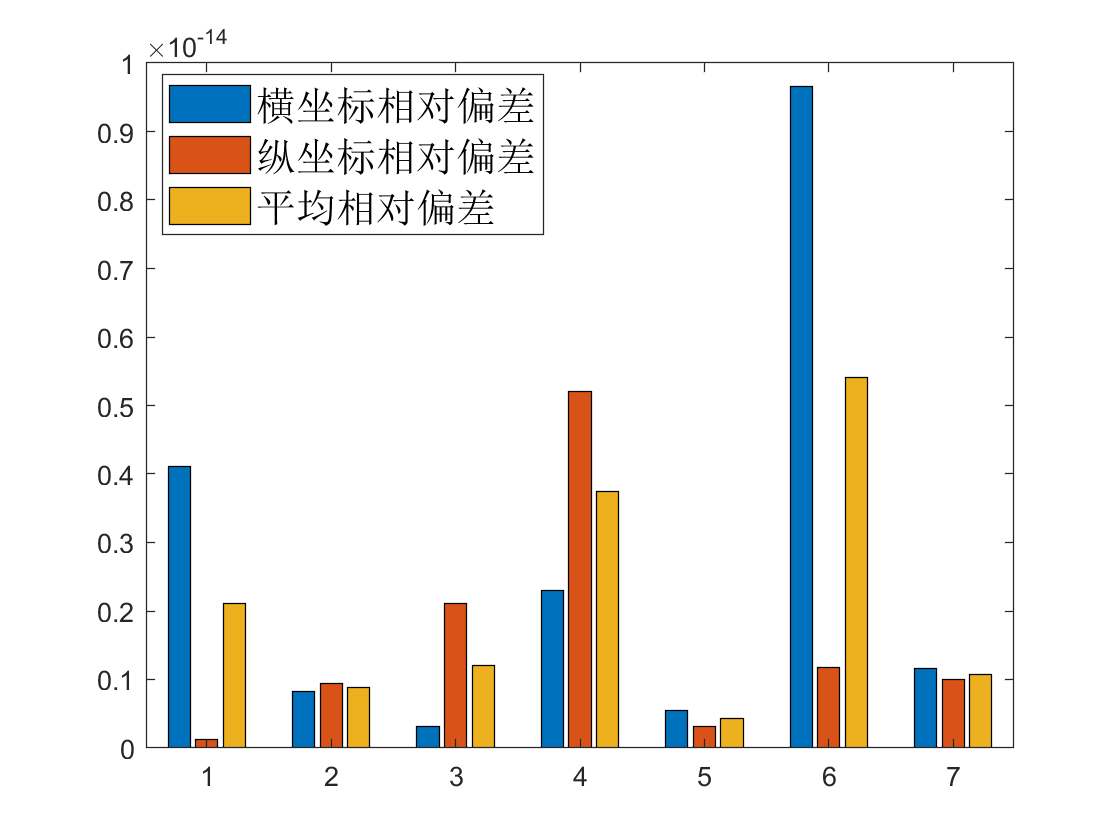
\includegraphics[width=0.7\textwidth]{e.png}
	\caption{相对误差条形图}
	\label{tux}
\end{figure}

\subsection{问题1.2的模型建立与求解}
继续假设$P$号无人机被动接收信号,其位置满足稍有偏差,FY00、FY01及另外若干编号未知的无人机发射信号,其位置无偏差。

当编号已知时,问题转化为问题1.1,即除了FY00、FY01之外,只需要额外一架无人机即可实现定位。当编号未知时,如果能通过角度的大小和相对关系确定具体的编号,问题即可解决。所以,问题(1.2)转化为使发射信号源编号确定所需的最少的无人机数目。

\subsubsection{均匀分布和圆心角、圆周角规律分析}
\textbf{5.2.1.1 飞行编队均匀分布的特性:}

由于九架无人机均匀地分布在圆上,每两架无人机之间的距离相等,且相邻两架无人机到FY00号无人机之间的夹角为$40^{\circ}$,任意两架无人机到FY00号无人机之间的夹角为$40n^{\circ}$($n$为整数)。
\begin{figure}[H]
	\centering
	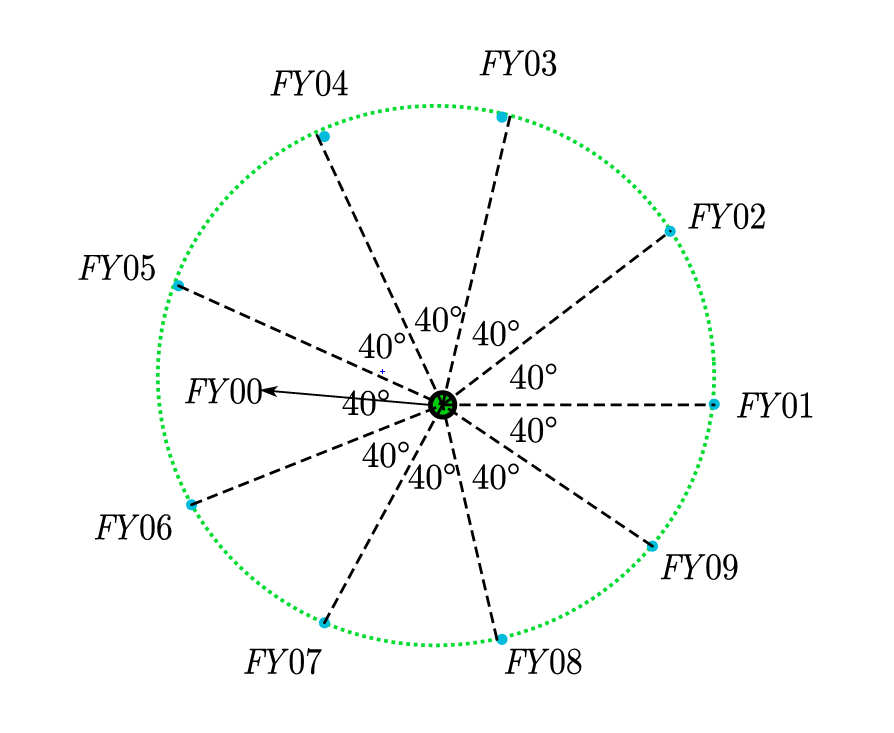
\includegraphics[width=0.7\textwidth]{均匀分布图.png}
	\caption{均匀分布示意图}
	\label{tu5}
\end{figure}

\textbf{5.2.1.2 两个无人机在圆周上时接收到夹角的角度规律:}

当两个在圆周上的无人机向接收信号的无人机发射信号时,夹角构成圆周角。根据圆周角为圆心角一半的特性,且圆心角均为$40n^{\circ}$($n$为整数),可知此类夹角一定是$20n^{\circ}$($n$为整数)。

\textbf{5.2.1.3 无人机FY00与任意编号无人机接收到夹角的角度规律:}

当无人机FY00与任意编号无人机向接收信号的无人机发射信号时,夹角构成圆周角。在下文图\ref{tu6}中分析其对应的圆心角的角度规律:

记接收源为点$P$,FY00为点$O$,FY01为点$A$,另外发射源在点为$B$。连结点$P$与原点$O$,延长并与圆相交于点$Q$。在图示特殊情况下,研究出FY00与另一个圆心上的无人机(这里是FY02)对应的夹角,$\angle{OPB}$为圆周角,对应圆心角为$\angle{QOB}$,可以看出圆心角$\angle{QOB}$为$20^{\circ}$的倍数且不是$40^{\circ}$的倍数,则
圆周角$\angle{OPB}$为$10^{\circ}$的倍数且不是$20^{\circ}$的倍数。

\begin{figure}[H]
	\centering
	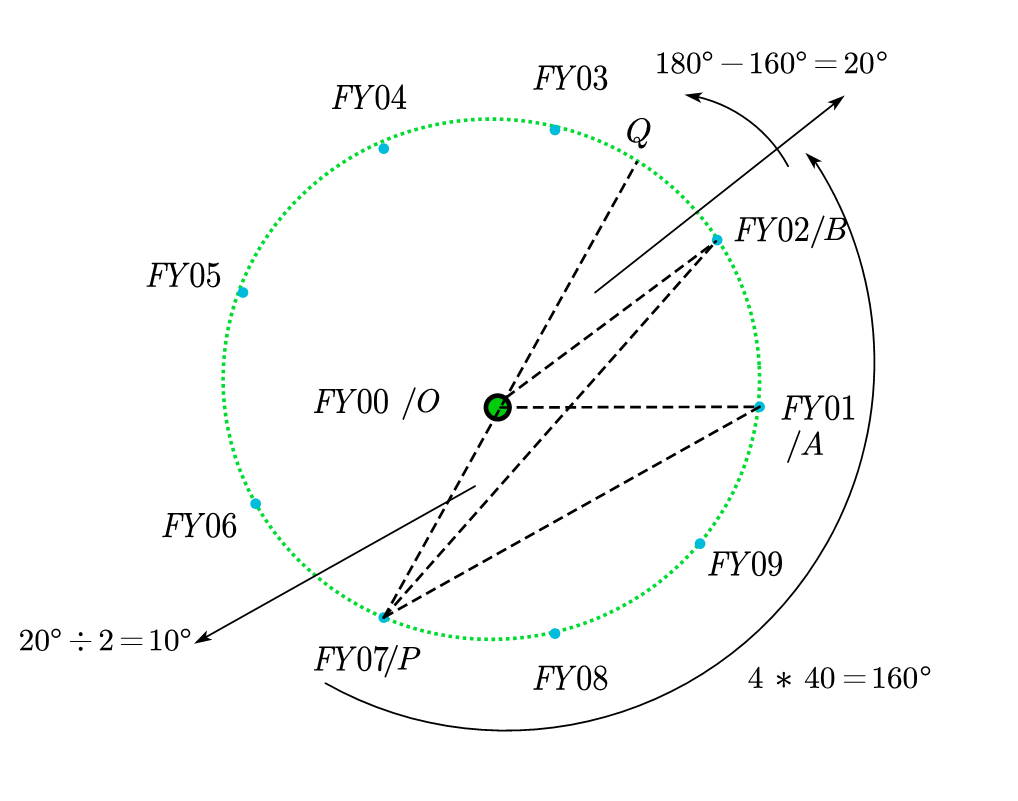
\includegraphics[width=0.6\textwidth]{20n+10.png}
	\caption{角度规律分析图}
	\label{tu6}
\end{figure}

在更一般的情形下,圆心角$\angle{QOB}=180^{\circ}-\angle{POA}=180^{\circ}-40n^{\circ}=40m^{\circ}+20^{\circ}$,则圆周角$\angle{OPB}=20m^{\circ}+10^{\circ}$。可以推出结论:无人机FY00与任意圆上无人机到接收源构成的夹角满足规律$20m^{\circ}+10^{\circ}$。

其中,$m,n$均为整数。

\textbf{5.2.1.4 角度规律总结:}

经过分析,角度规律可以总结为:圆周上两无人机与接收源形成角$20n^{\circ}$($n$为整数);圆周上一无人机、无人机FY00与接收源形成角$20m^{\circ}+10^{\circ}$($m,n$为整数)

根据题意:编号为FY00、FY01的无人机及若干编号未知的无人机发射信号。当需要确定编号的额外无人机为一架时,三个角分别为$20n^{\circ}$、$20m_1^{\circ}+10^{\circ}$、$20m_2^{\circ}+10^{\circ}$;当需要确定编号的额外无人机为两架时,六个角分别为$20n_1^{\circ}$、$20n_2^{\circ}$、$20n_3^{\circ}$、$20m_1^{\circ}+10^{\circ}$、$20m_2^{\circ}+10^{\circ}$、$20m_3^{\circ}+10^{\circ}\cdots$

其中,$m_i,n_i$均为整数。

\subsubsection{添加一个额外发射源确定无人机编号}
下面考虑仅通过添加一个额外发射源确定各无人机编号的方法。根据规律分析的结论,已知三个角的角度形式为:$20n^{\circ}$、$20m_1^{\circ}+10^{\circ}$、$20m_2^{\circ}+10^{\circ}$($m_1,m_2,n$均为整数)。

将此时的接收无人机记为$k$,发射信号的无人机编号为0,1,$i$,记无人机$01,0i,1i$对应的夹角$\alpha_{01},\alpha_{0i},\alpha_{1i}$,接收到三个夹角为$\alpha_{1},\alpha_{2},\alpha_{3}$。

\textbf{5.2.2.1 分析$\alpha_{01}$:}

$\alpha_{01}$为无人机发射源FY00、FY01及接收信号的无人机$k$形成的夹角。接收信号的无人机知晓自己的编号$k$,由编号$k,0,1$可以求出理想情况下夹角$\alpha_{01}^{*}$的值。

求解方法如图\ref{tu7}所示:
\begin{figure}[H]
	\subfigure{
		\begin{minipage}{0.5\textwidth}
			\centering
			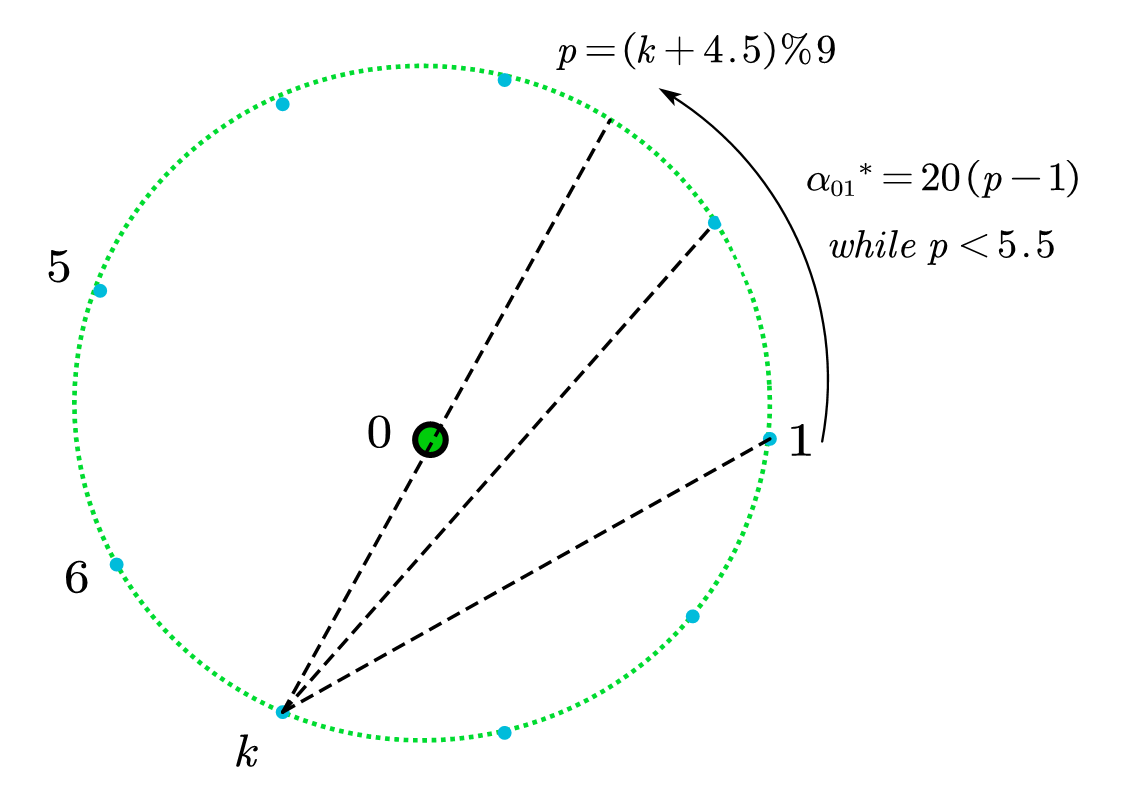
\includegraphics[width=1.0\textwidth]{p情况1.png}
		\end{minipage}
	}
	\subfigure{
		\begin{minipage}{0.5\textwidth}
			\centering
			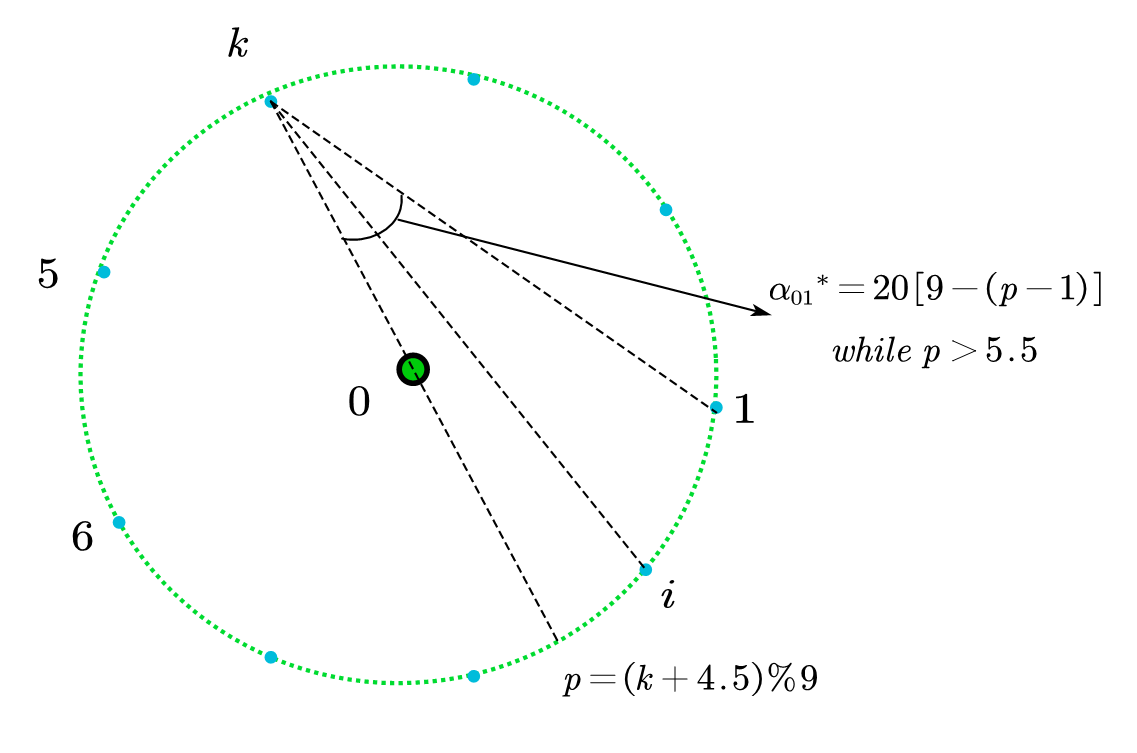
\includegraphics[width=1.0\textwidth]{p情况2.png}
		\end{minipage}
	}
	\caption{$\alpha_{01}^{*}$的求解}
	\label{tu7}
\end{figure}

延长接收源与圆心的连线交圆于某点$Q$。记$p=(k+4.5)\%9$为点$Q$的虚拟编号,虚拟编号的值表示点$Q$在编号$[p]$对应点至编号$[p]+1$对应点相连圆弧的中间位置。编号夹角$\alpha_{01}^{*}$的值转化为编号$p$、编号$1$与接收源编号$k$的点形成的夹角。

此时存在两种情况:

(1)当编号$p<5.5$时,$20(p-1)$对应劣弧的度数,满足条件;

(2)当编号$p>5.5$时,$20(p-1)$对应优弧的度数,需要转化为劣弧的度数,才能与接收的信息吻合,此时$\alpha_{01}^{*}=20(9-(p-1))$。

于是,求得$\alpha_{01}$的理想解$\alpha_{01}^{*}$。下面根据理想解匹配得到$FY00$、$FY01$与接收点之间形成的夹角$\alpha_{01}$。
$$ Min \quad S_1=|\alpha_{01}^{*}-\alpha_{k_1}| $$
\begin{equation}
	s.t.
	\begin{cases}
		k_1\in{\{1,2,3\}}	\\
		|\alpha_{01}^{*}-\alpha_{k_1}|<Maxerror
	\end{cases}
\end{equation}

其中,$k_1$表示$\alpha_{k_1}=\alpha_{01}$,即接收到的夹角信息,$\alpha_{k_1}^{*}$表示当接收点位于理想位置时应该接受到的夹角信息,$Maxerror$表示允许的误差限。

于是匹配可以得到$\alpha_{1}$的实际解$\alpha_{k_1}$,也可得到$\alpha_{1},\alpha_{2},\alpha_{3}$与$\alpha_{01},\alpha_{0i},\alpha_{1i}$中的其中一对对应关系,只需再确定一对对应关系及求出$i$,即可求解。

\textbf{5.2.2.2 求解编号$i$:}

(1)根据角度形式明确所有角的对应关系:

根据角度规律的分析,$\alpha_{1i}=20n$($n$为整数),现有剩余的两个角形式分别为$20n^{\circ},20m^{\circ}+10^{\circ}$,则可以确定$\alpha_{1i}$的值。
$$ Min \quad S_2=|\alpha_{k_2}-20n| $$
\begin{equation}
	s.t.
	\begin{cases}
		k_2\in{\{1,2,3\}}	\\
		k_2\neq k_1 \\
		|\alpha_{k_2}-20n|<Maxerror
	\end{cases}
\end{equation}

其中,$k_2$表示$\alpha_{k_2}=\alpha_{1i}$,即接收到$1,i$对应的夹角信息,$Maxerror$表示允许的误差限。

此时找到了第二对对应关系,只需求出$i$即可明确任意信号发射源的编号及任意两个发射源所对应的夹角。

(1)根据$1,i$夹角得到$i$的两个解$i_1,i_2$:

对$1,i$对应的夹角进行分析,即可得到如下关系式:
\begin{equation}
	\begin{cases}
		\alpha_{k_2}=20(k_2-1)	   & k_2=2,3,4,5\\
		\alpha_{k_2}=20(9-(k_2-1)) & k_2=6,7,8,9
	\end{cases}
\end{equation}

(2)根据$0,i$夹角得到$i$的两个解$i_3,i_4$:

分析$0,i$对应夹角,类似于分析$0,1$对应的夹角,得到如下关系式:
\begin{equation}
	\begin{cases}
		\alpha_{k_3}=20(p-i)	   & k_3=2,3,4,5\\
		\alpha_{k_3}=20(9-(p-i))   & k_3=6,7,8,9
	\end{cases}
\end{equation}

其中,$k_3$表示$\alpha_{k_3}=\alpha_{0i}$,即接收到的$0,i$对应夹角信息,$p=(k+4.5)\%9$,表示虚拟编号$Q$的值(见前文图\ref{tu7}所示。

(3)最终确定编号$i$:
显然,真实的$i$值在集合$\{i_1,i_2\}$与集合$\{i_3,i_4\}$的交中一定存在;但是如果存在:$i_1=i_3,i_2=i_4$或者$i_1=i_4,i_2=i_3$的情况,即存在两组解,依然无法确定最终解。

下图\ref{tu8}说明了这种情况不可能发生:
\begin{figure}[H]
	\centering
	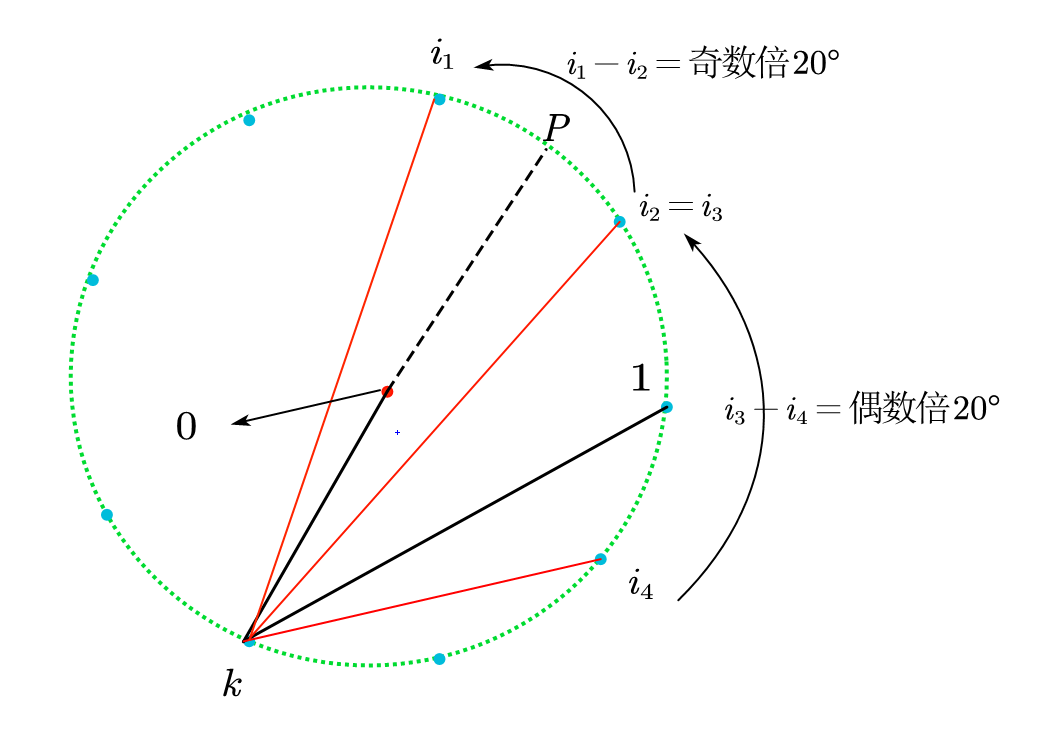
\includegraphics[width=0.6\textwidth]{唯一解证明.png}
	\caption{$i$的唯一性分析图}
	\label{tu8}
\end{figure}

$i_1$和$i_2$关于线段$OP$对称,则对应圆心角为奇数倍个$20^{\circ}$;$i_3$和$i_4$关于0和1位置的连线对称,则对应圆心角为偶数倍个$20^{\circ}$;当$i_2=i_3$时,$i_1$一定不等于$i_4$,即不存在两个解。最终解为:$i=\{i_1,i_2\}\cup\{i_3,i_4\}$。

\textbf{5.2.2.3 结论:}

发射源FY00、FY01和圆周上任意一架无人机发射信号,可以通过分析角度关系求出未知编号无人机的编号,并得到三个角与分别与两个发射源的对应关系。

\subsubsection{模型求解与检验}
设计验证模式:已知编号FY00、FY01和编号$i$(令$i=2$进行验证)的无人机发射信号,自定义满足条件的数据,使得接受信号无人机位置稍有偏差,依次选择其他无人机验证求解编号$i$的值,与给定$i$的值进行比较验证。求解结果见表格\ref{b1},结果显示上述求解未知编号的方法可行、正确。

\begin{table}[H]
	\centering
	\caption{求解编号验证表}
	\begin{tabular}{ccccccccc}
		\toprule[1.5pt]
		发射   & 接收 & $\alpha_1$   & 对应发点 & $\alpha_2$   & 对应发点 & $\alpha_3$    & 对应发点 & 逆推编号 \\ 
		\midrule[1pt]
		\multirow{7}{*}{0,1,2} & 3     & 45.88249 & 9,0   & 56.72687 & 9,1   & 10.84437 & 0,1   & 2                      \\ \cline{2-9} 
		& 4     & 38.85423 & 9,1   & 25.55319 & 9,0   & 13.30104 & 0,1   & 2                      \\ \cline{2-9} 
		& 5     & 32.2266  & 2,1   & 14.11228 & 0,1   & 18.11432 & 2,0   & 2                      \\ \cline{2-9} 
		& 6     & 25.8194  & 2,1   & 11.71116 & 0,1   & 14.10823 & 2,0   & 2                      \\ \cline{2-9} 
		& 7     & 22.4301  & 2,1   & 8.44134  & 0,1   & 13.98876 & 2,0   & 2                      \\ \cline{2-9} 
		& 8     & 19.68821 & 2,1   & 6.467809 & 0,1   & 13.2204  & 2,0   & 2                      \\ \cline{2-9} 
		& 9     & 17.12872 & 2,1   & 6.050137 & 0,1   & 11.07858 & 2,0   & 2                      \\ 
		\bottomrule[1.5pt]
	\end{tabular}
\end{table}

注:$Matlab$中用1表示编号为FY00的无人机,编号2在$Matalb$中表示为3。

\subsection{问题1.3的模型建立与求解}
\subsubsection{模型的建立}
无人机编队均匀分布在半径$r=100$米的圆上或位于圆心,通过FY00与圆周上最多三架无人机发射信号,帮助编队中的其他无人机确定自身的位置。

分析可知:

(1)理论上,除圆心外圆周上需要的无人机架数至少为两架;由题意,圆周上的无人机架数为两架或三架;

(2)在初始位置数据中,满足位于理想位置的无人机为FY00、FY01,共两架;

(3)接收信号的无人机无法得知发射信号无人机的实际坐标,只能以发射信号无人机的理想坐标进行定位,于是产生了定位误差,需要通过迭代多次调整求得误差更小的解;

(4)由于已知无人机编号及理想位置,可以求得每架无人机与理想位置的距离来衡量误差,下一轮可以选择误差最小的三或四个点进行定位。

(5)FY00、FY01位置无误差,每次固定选择这两个点,再另外选择一个或两个距离与理想距离最小的无人机发射信号。

使用问题1.1中建立的模型进行求解,每次除FY00、FY01额外选取一个点误差最小的点进行定位。求解过程可以用流程图表示,见图\ref{tu9}:
\begin{figure}[H]
\centering
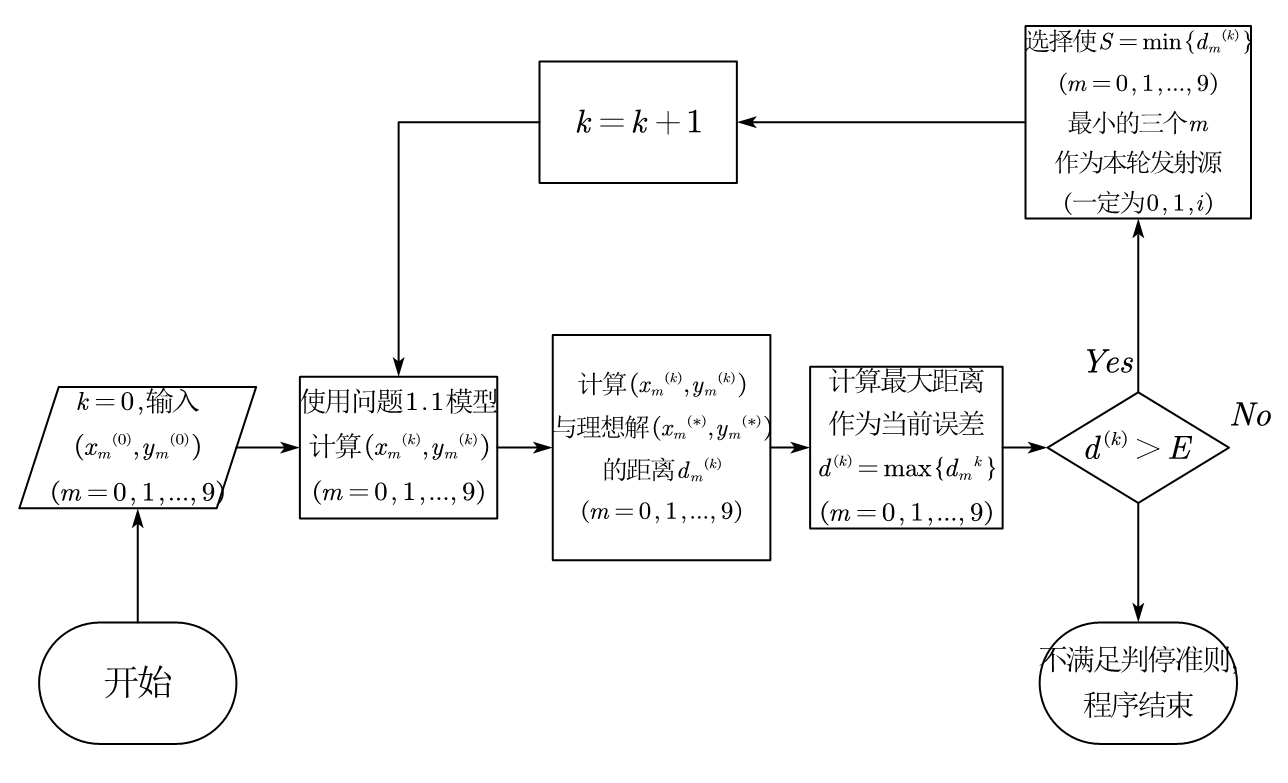
\includegraphics[width=1.0\textwidth]{1.3模型求解流程图.png}
\caption{模型求解流程图}
\label{tu9}
\end{figure}

第$k$轮迭代第$m$架无人机的误差:
\begin{equation}
	d_m^{k}=\sqrt{(x_m^{k}-x_m^{*})^2+(y_m^{k}-y_m^{*})^2} \quad m=0,1,2...,9
\end{equation}

第$k$轮迭代的误差:
\begin{equation}
	d^{k}=Max\{d_m^{*}\} \quad m=0,1,2...,9
\end{equation}

其中,$(x_m^{(k)},y_m^{(k)})$表示第$k$次迭代求出的编号为$m$的无人机的位置,$(x_m^{(*)},y_m^{(*)})$表示编号为$m$的无人机的理想位置,$d_m^{k}$表示第$k$次迭代求出的编号为$m$的无人机与理想位置的距离,$d^{k}$表示第$k$次迭代求出的所有无人机与理想位置的最大距离,能够容忍的最大距离平方为$E$。

\subsubsection{模型的求解}
按照流程图所示的方法求解,令容忍的最大距离平方为$E^2=0.01$,可以通过五次迭代实现调整。五次迭代的误差下降图和无人机分布图,分别为图\ref{tu10}及图\ref{tu11}。

\begin{figure}[H]
	\centering
	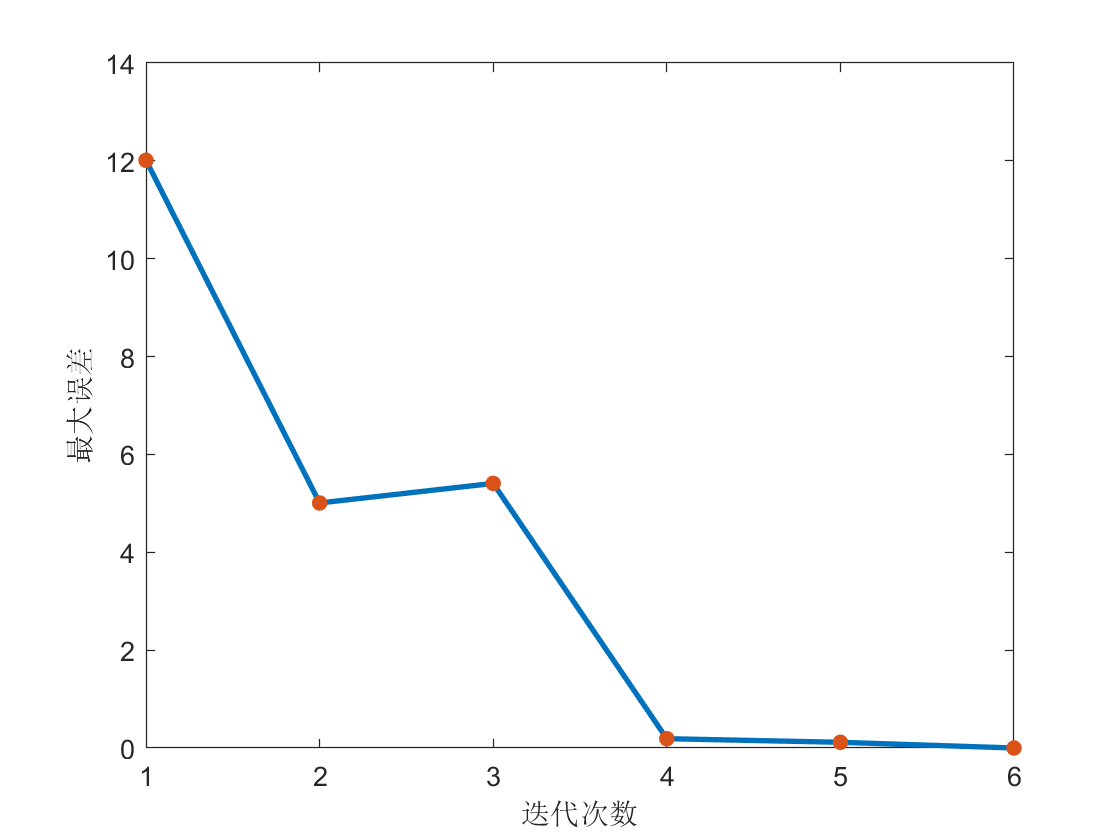
\includegraphics[width=0.7\textwidth]{误差折线图.png}
	\caption{误差折线图}
	\label{tu10}
\end{figure}

\begin{figure}[H]
	\subfigure{
		\begin{minipage}{0.5\textwidth}
			\centering
			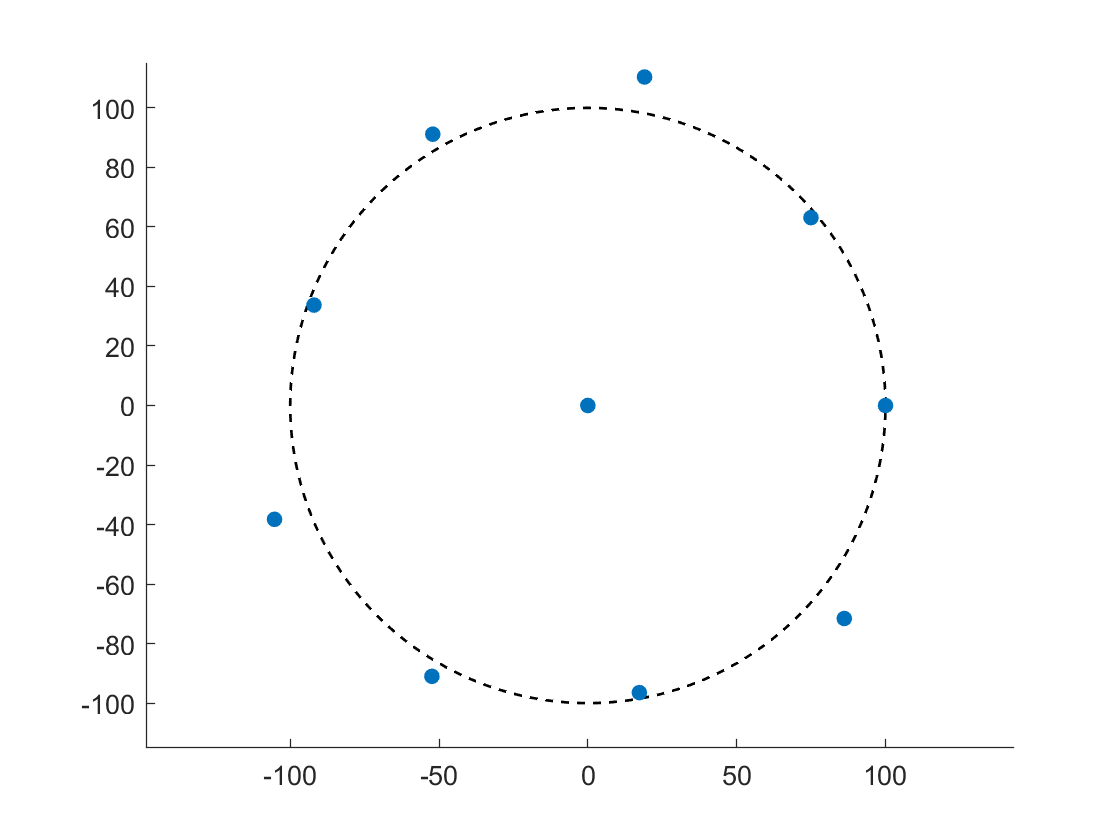
\includegraphics[width=1.0\textwidth]{三一.png}
		\end{minipage}
	}
	\subfigure{
		\begin{minipage}{0.5\textwidth}
			\centering
			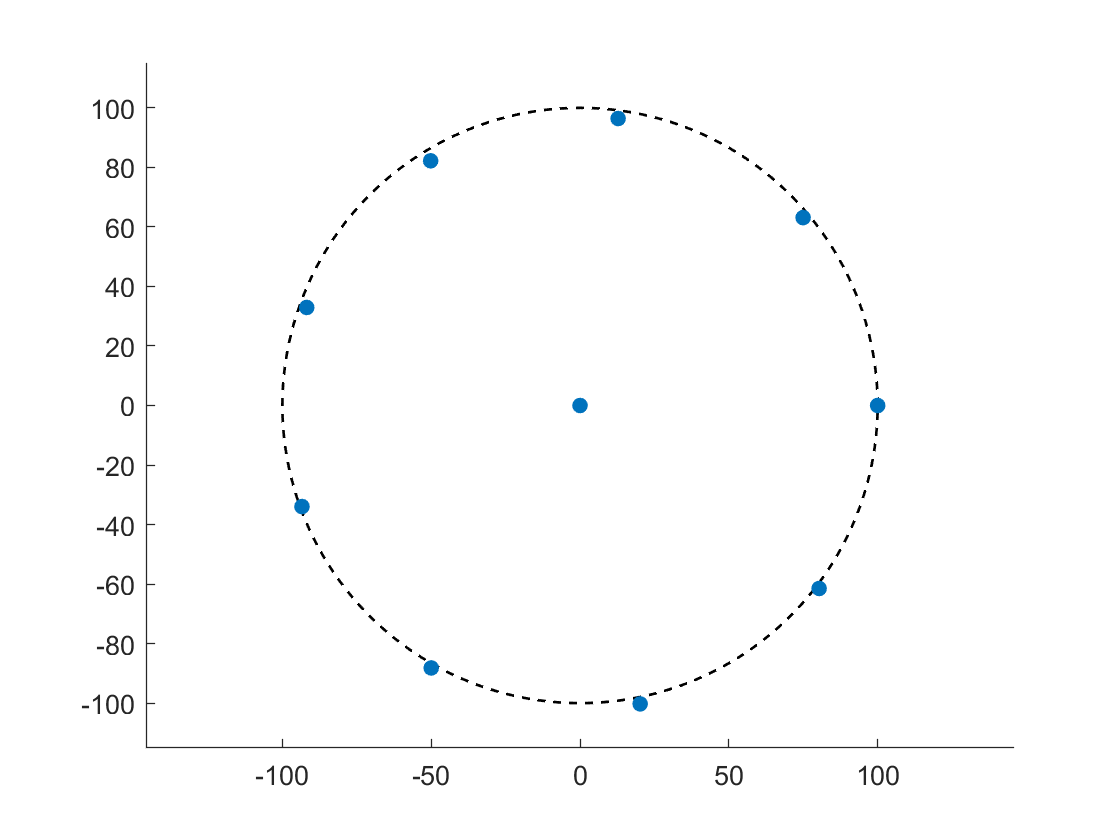
\includegraphics[width=1.0\textwidth]{三二.png}
		\end{minipage}
	}
	\subfigure{
		\begin{minipage}{0.5\textwidth}
			\centering
			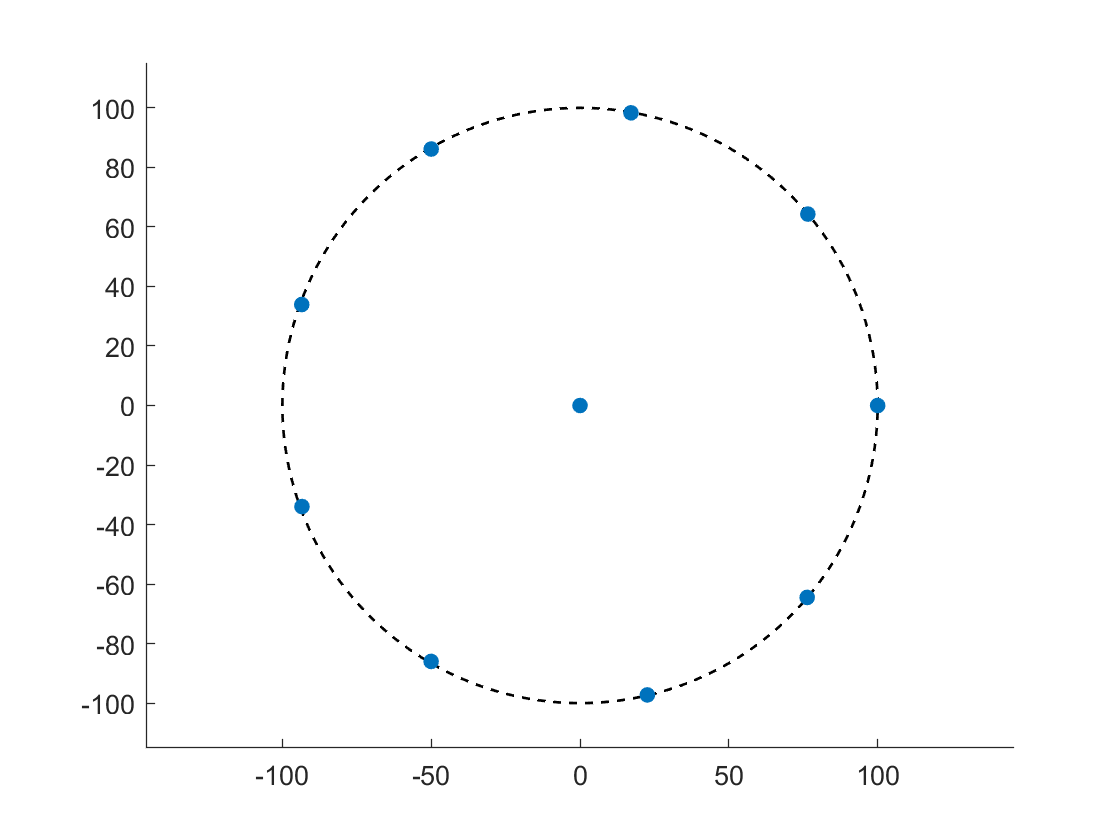
\includegraphics[width=1.0\textwidth]{三三.png}
		\end{minipage}
	}
	\subfigure{
		\begin{minipage}{0.5\textwidth}
			\centering
			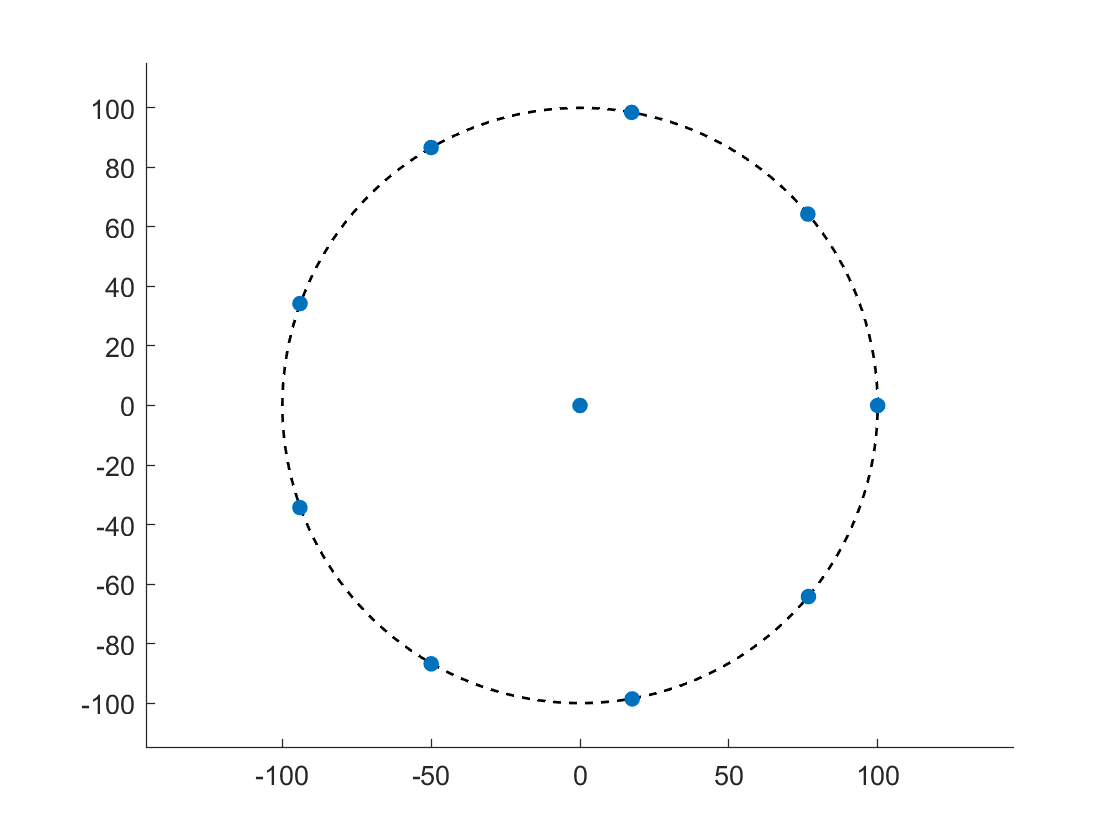
\includegraphics[width=1.0\textwidth]{三四.png}
		\end{minipage}
	}
	\subfigure{
		\begin{minipage}{0.5\textwidth}
			\centering
			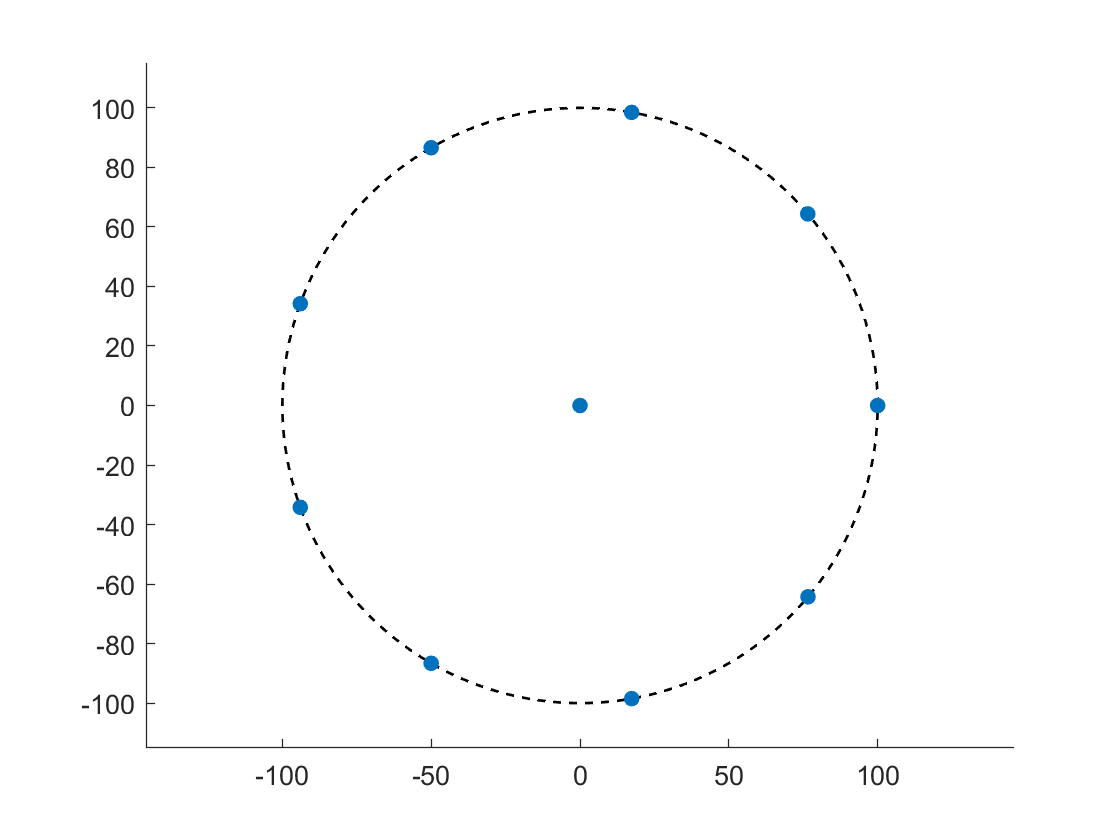
\includegraphics[width=1.0\textwidth]{三五.png}
		\end{minipage}
	}
	\subfigure{
		\begin{minipage}{0.5\textwidth}
			\centering
			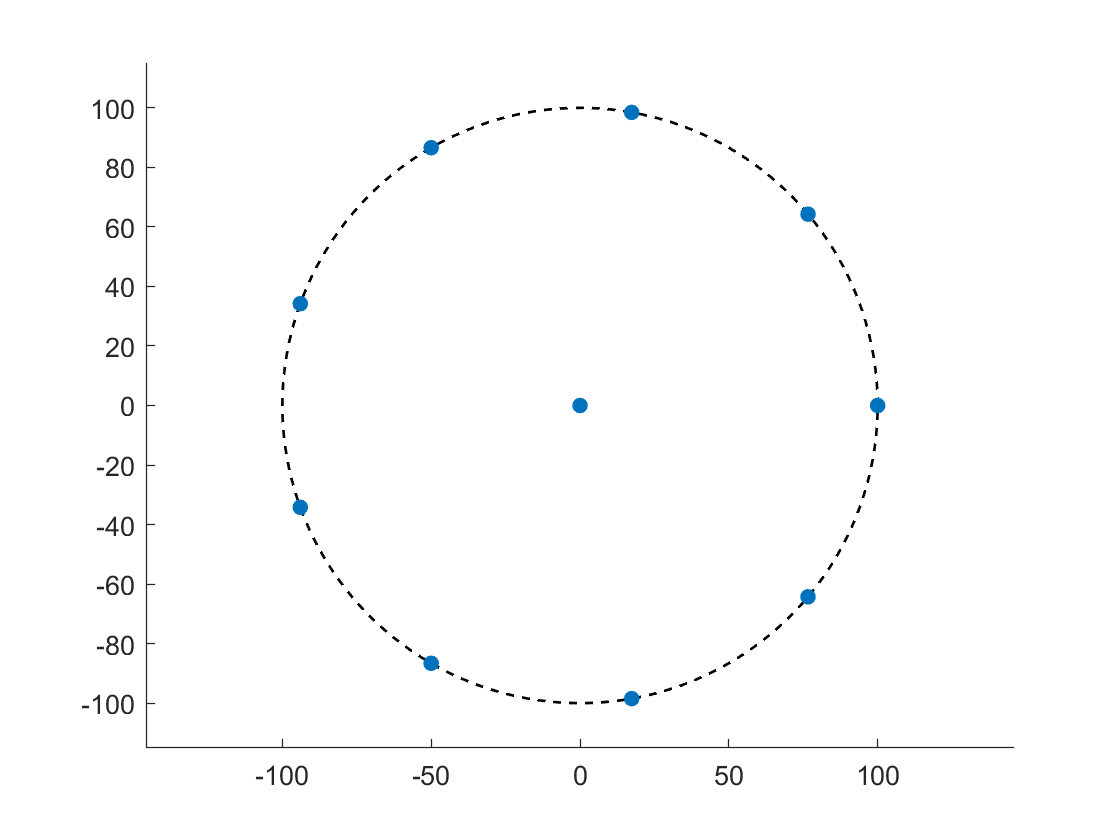
\includegraphics[width=1.0\textwidth]{三六.png}
		\end{minipage}
	}
	\caption{迭代调整过程图}
	\label{tu11}
\end{figure}
由图\ref{tu11},迭代过程的调整过程图可知,在第一次和第二次迭代的结果显示了肉眼可见的误差;而当到达第三次之后,误差已经无法明显观察到接近于0,说明模型可行性及精度;而观察误差折现图\ref{tu11},当到达第4次时,误差已经接近于0,说明问题已经基本解决,模型精度高。

\subsection{问题2的模型建立与求解}
\subsection{模型建立}
问题2考虑锥形编队无人机队形,直线上相邻两架无人机间距为50$m$。

(1)假设该编队中接收信号的无人机与问题1中情形相似,均与理想距离稍有偏差;

(2)由问题1.1的分析可知,只需要一个圆心和两个该圆上的点即可对其他圆上的点进行定位;

(3)由问题1.3的分析可知,当一个圆通过锥形编队中至少三个点时,能够知道圆心和圆上一个点的理想位置且其他位置稍有偏差时,可以通过问题1.3的模型能够将该圆上的所有点的坐标调整至理想位置;

(4)该锥形编队,可以通过相互之间存在相交关系的若干圆进行覆盖;

问题转化为在锥形编队中构造圆形编队,向周围不同的圆发散求解,每次只有三架无人机发射信号,位于同一个圆上的其他无人机接收信号,确定部分无人机的位置,然后确定其他圆上的无人机的位置。
求解顺序的演示图\ref{tu13}:

\begin{figure}[H]
	\subfigure{
		\begin{minipage}{0.6\textwidth}
			\centering
			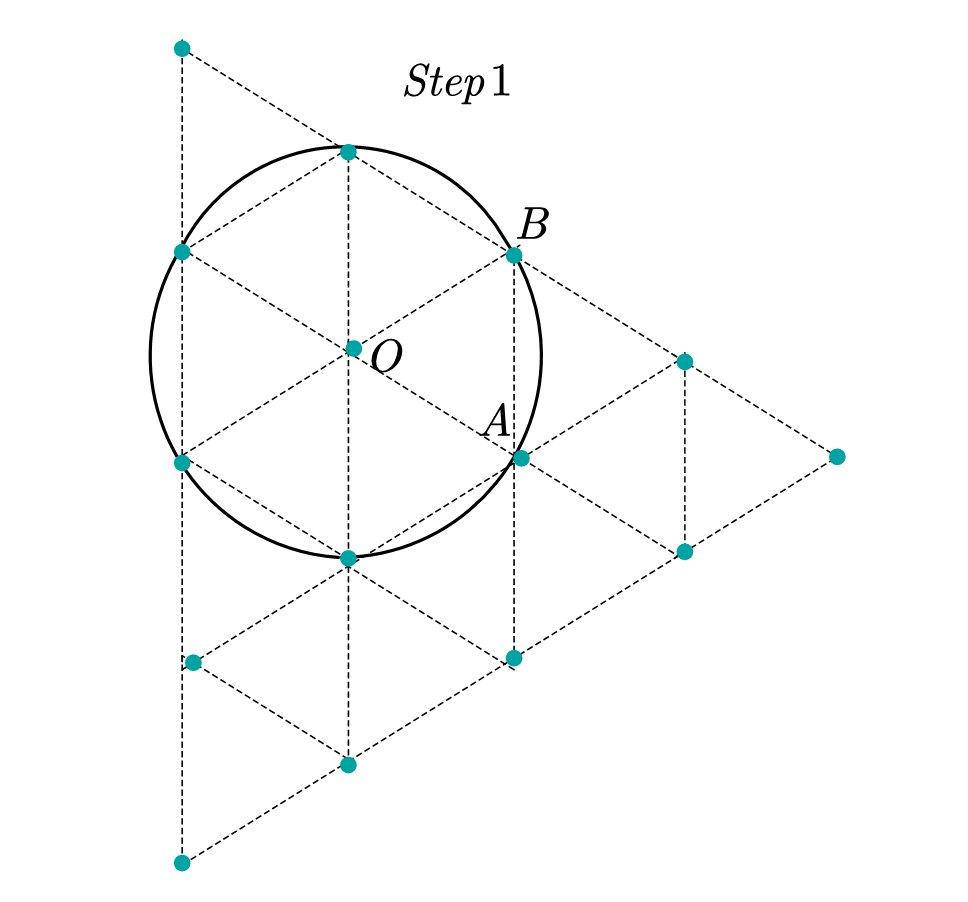
\includegraphics[width=1.0\textwidth]{问题2.1.png}
		\end{minipage}
	}
	\subfigure{
		\begin{minipage}{0.5\textwidth}
			\centering
			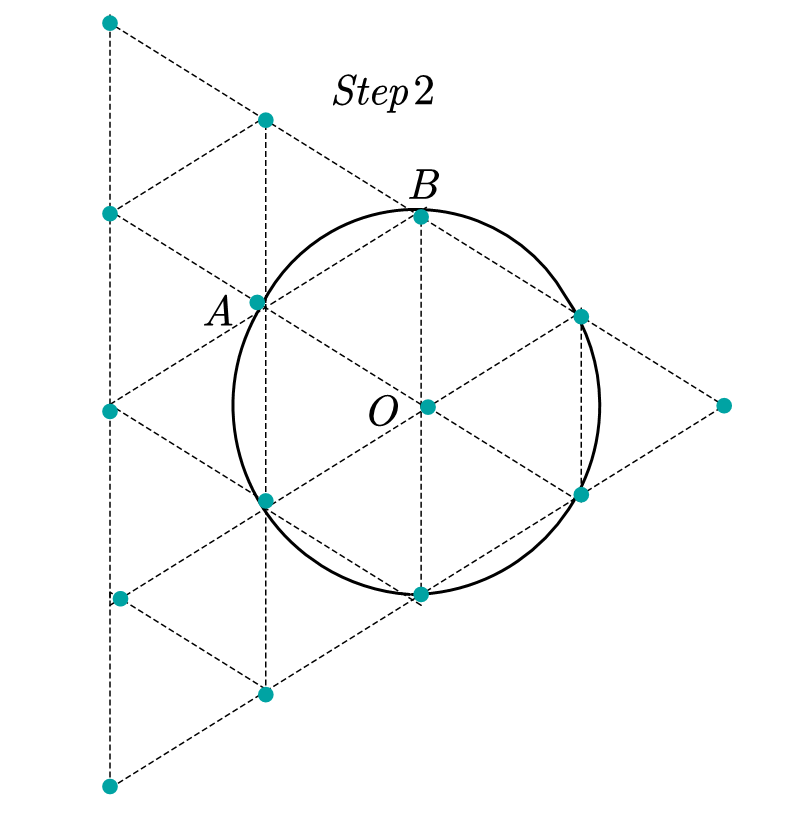
\includegraphics[width=1.0\textwidth]{问题2.2.png}
		\end{minipage}
	}
	\caption{问题2求解模型过程图1-2}
	\label{tu13}
\end{figure}

\begin{figure}[H]
	\subfigure{
		\begin{minipage}{0.5\textwidth}
			\centering
			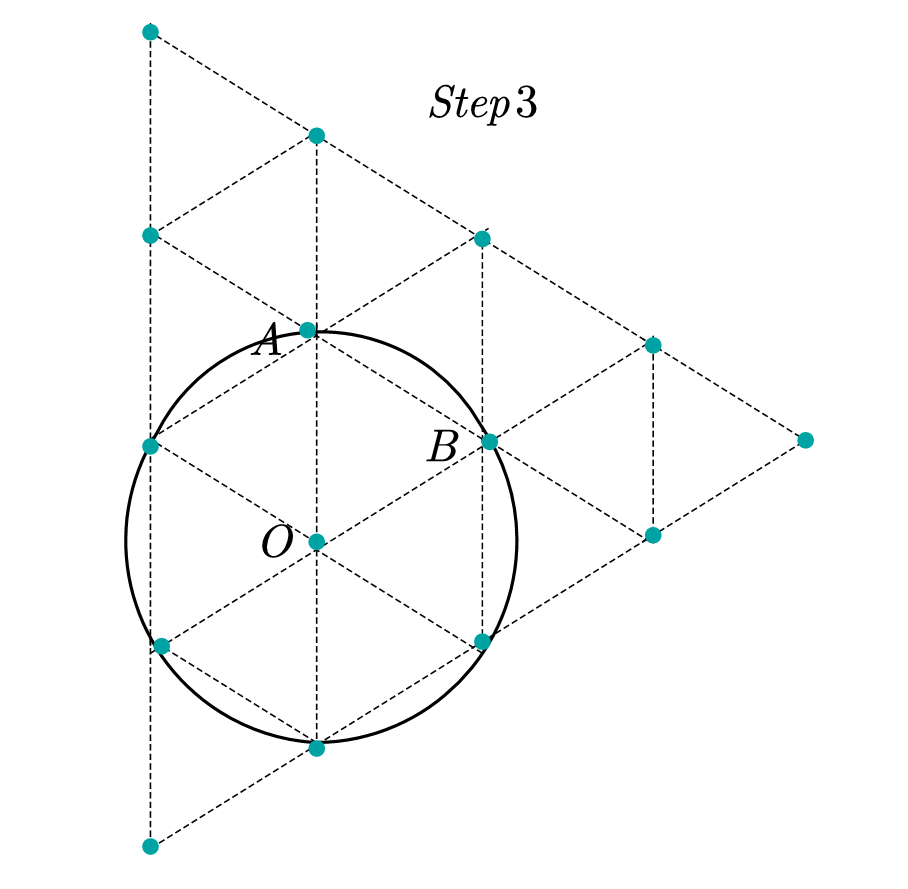
\includegraphics[width=1.0\textwidth]{问题2.3.png}
		\end{minipage}
	}
	\subfigure{
		\begin{minipage}{0.5\textwidth}
			\centering
			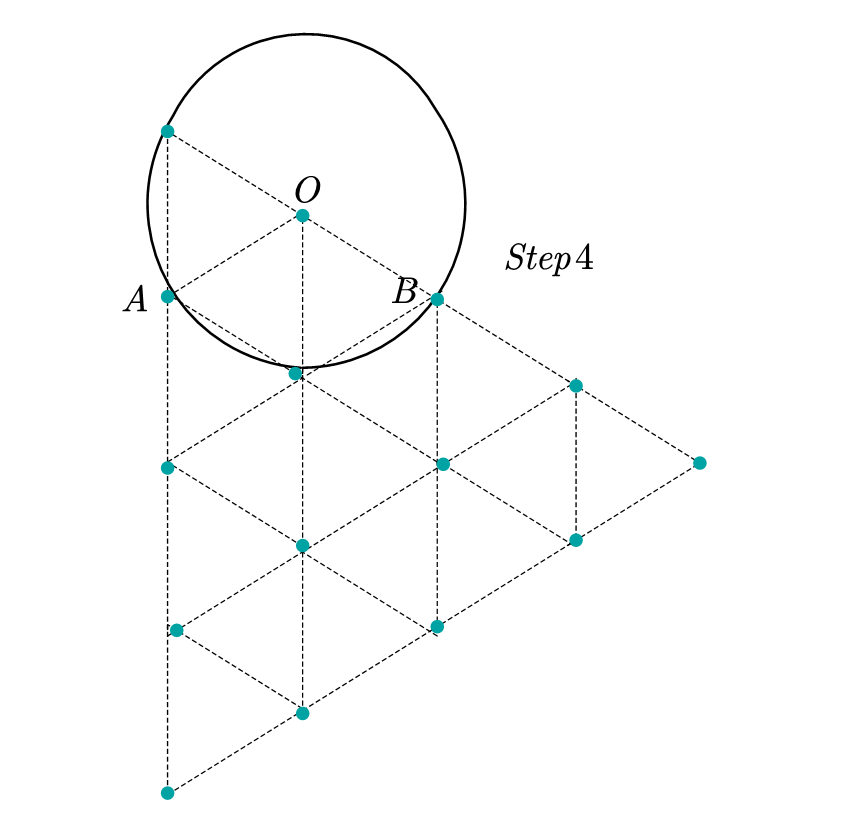
\includegraphics[width=1.0\textwidth]{问题2.4.png}
		\end{minipage}
	}
	\subfigure{
	\begin{minipage}{0.5\textwidth}
		\centering
		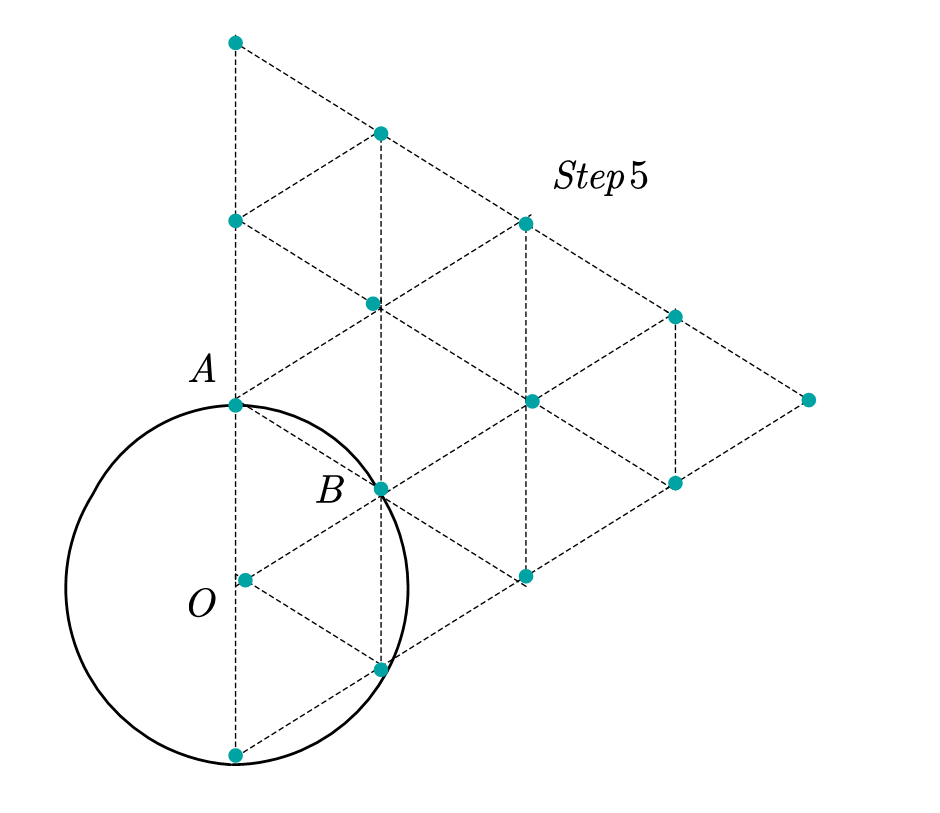
\includegraphics[width=1.0\textwidth]{问题2.5.png}
	\end{minipage}
	}
	\subfigure{
	\begin{minipage}{0.5\textwidth}
		\centering
		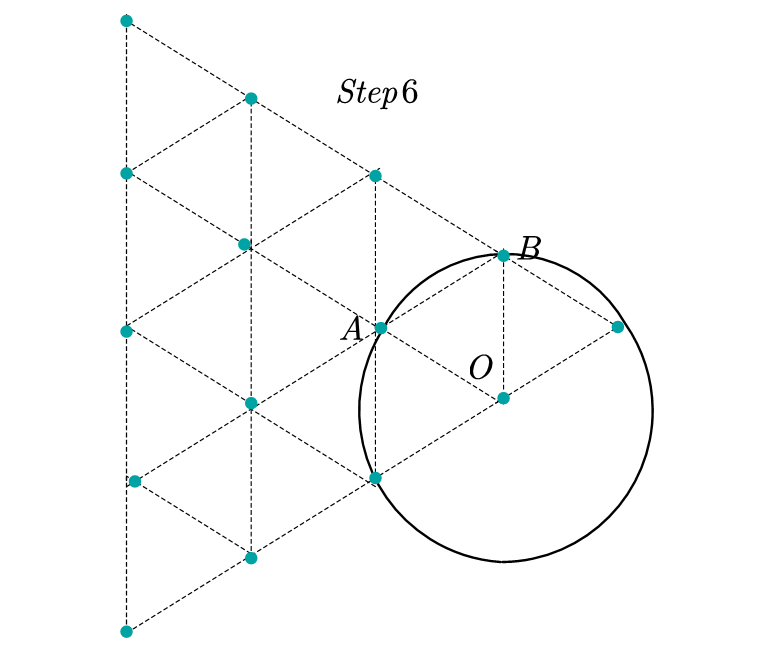
\includegraphics[width=1.0\textwidth]{问题2.6.png}
	\end{minipage}
	}
	\caption{问题2求解模型过程图4-6}
	\label{tu14}
\end{figure}

\subsection{模型求解及检验}
建系:这里假设直
线上相邻两架无人机的间距相等为200米,以1为原点,1到5的方向为正方向,初始精确点定位$Step1$图中的$O,A$点。

建立锥形定位模型,编号信息见图\ref{tu16},检验的误差图见图\ref{tu17}。

\begin{figure}[H]
	\centering
	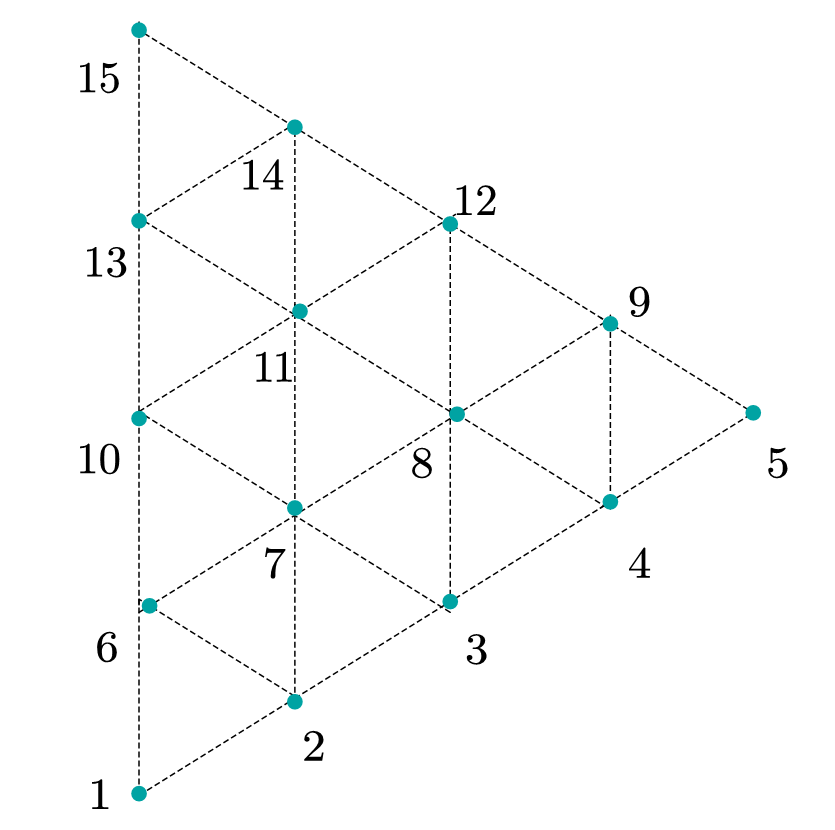
\includegraphics[width=0.7\textwidth]{锥形图.png}
	\caption{锥形图}
	\label{tu16}
\end{figure}

\begin{figure}[H]
	\centering
	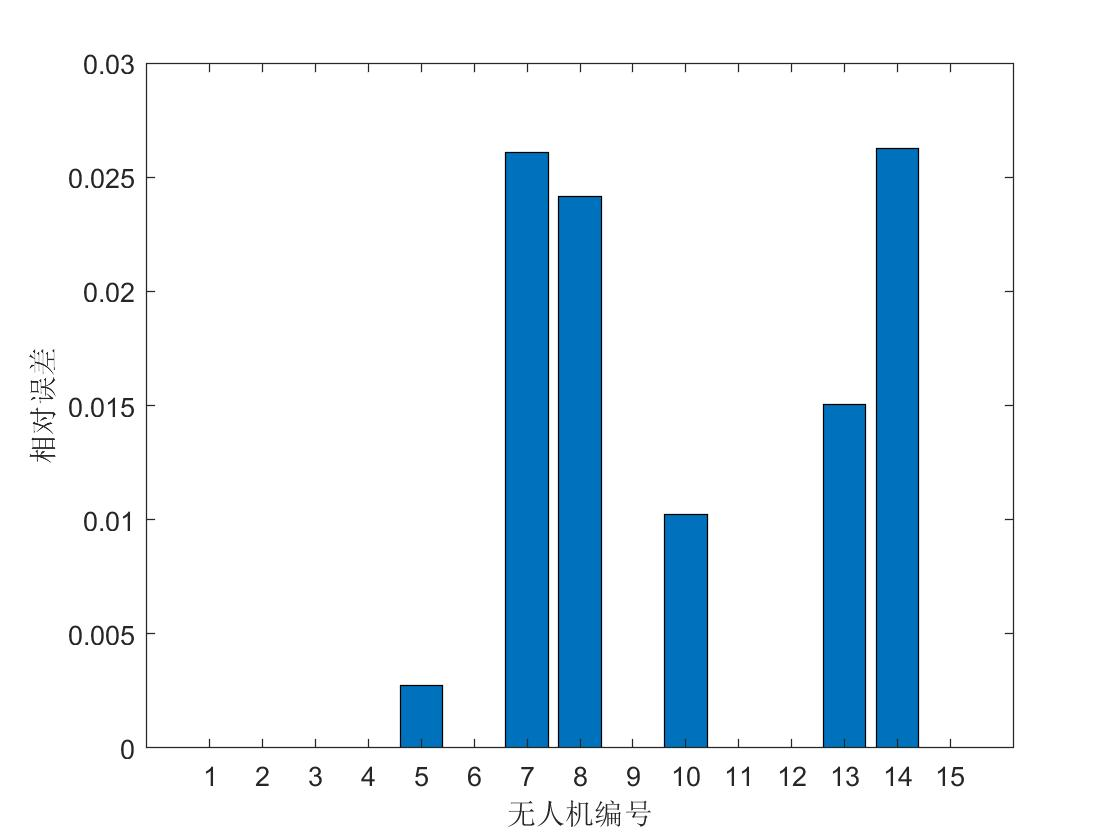
\includegraphics[width=0.7\textwidth]{45.jpg}
	\caption{问题2误差图}
	\label{tu17}
\end{figure}

\section{优缺点分析}
\subsection{优点}
(1)理想解的运用:通过分析实际解与理想解的距离,可以将求解限制在某一领域内。于是可以通过将理想解赋为初值,运用$Matlab$的$vpasolve$函数结合初值,快速求出解;

(2)通过分析几何关系,将问题1.2转化为了问题1.1,简化了模型的求解难度;

(3)通过分析锥形的几何特征,利用六个圆覆盖锥形上的15个点,从而将该问题转化为问题1.3。

\subsection{缺点}
夹角余弦方程组的求解有一定的不稳定性,给求解代码的书写带来了不小的难度。

% 参考文献
\bibliography{book} % 采用外面导入bib文件形式

\newpage

% 附录
\appendix
\ctexset{
	section={
		format=\zihao{-3} \heiti \centering,
		name = {附录,},
		number = \Alph{section},
		aftername=\hspace{12pt},
	}
}

\section{通用函数1}
\begin{lstlisting}[title="comp\_alpha.m",language=matlab]
% 代码段
function output = comp_alpha(x1y1,x2y2,x3y3,xy)
% 约定1-2之间的夹角是alpha1,2-3之间的夹角是alpha2,1-3之间的夹角是alpha3
[inner_product1,mod1] = inner_product_model(x1y1,x2y2,xy);
[inner_product2,mod2] = inner_product_model(x2y2,x3y3,xy);
[inner_product3,mod3] = inner_product_model(x1y1,x3y3,xy);
alpha1 = acos(inner_product1/mod1);
alpha2 = acos(inner_product2/mod2);
alpha3 = acos(inner_product3/mod3);
output = [alpha1,alpha2,alpha3];
end
\end{lstlisting}

\section{通用函数2}
\begin{lstlisting}[title="inner\_product\_model.m",language=matlab]
% 代码段
function output = comp_alpha(x1y1,x2y2,x3y3,xy)
% 约定1-2之间的夹角是alpha1,2-3之间的夹角是alpha2,1-3之间的夹角是alpha3
[inner_product1,mod1] = inner_product_model(x1y1,x2y2,xy);
[inner_product2,mod2] = inner_product_model(x2y2,x3y3,xy);
[inner_product3,mod3] = inner_product_model(x1y1,x3y3,xy);
alpha1 = acos(inner_product1/mod1);
alpha2 = acos(inner_product2/mod2);
alpha3 = acos(inner_product3/mod3);
output = [alpha1,alpha2,alpha3];
end
\end{lstlisting}

\section{问题1.1源代码1}
\begin{lstlisting}[title="shumo\_B\_1\_12.m",language=matlab]
function output = shumo_B_1_12(input1,input2,input3,input4,input5,input6,input7)
% 3个发送位置的坐标
FYsend1 = input1; % 圆心 直角坐标
FYsend2 = input2; % FY01
FYsend3 = input3; % FY02
FYsend = [FYsend1;FYsend2;FYsend3];

% 接收信息,只有三个角度的大小信息
alpha1 = input4; % 弧度
alpha2 = input5;
alpha3 = input6;

% 找到所有可能的情况
FYsend_perm = perms([1 2 3]); % 给出1 2 3这三个发射位置编号的排列
n = size(FYsend_perm,1);
error = +inf; % 设定所求出的位置和目标位置误差的初始值为正无穷
temp_xy = []; % 记录FYsend_perm中误差最小的情况对应位置

syms x y
ini = input7; % 设定初值为目标位置
for i = 1:n
temp_xy_code1 = FYsend_perm(i,[1 2]); % alpha1对应的两个发射点编号
temp_xy_1_1 = FYsend(temp_xy_code1(1),:);
temp_xy_1_2 = FYsend(temp_xy_code1(2),:);
[inner_product1,model1] = inner_product_model(temp_xy_1_1,temp_xy_1_2,[x y]);

temp_xy_code2 = FYsend_perm(i,[2 3]); % alpha2对应的两个发射点编号
temp_xy_2_1 = FYsend(temp_xy_code2(1),:);
temp_xy_2_2 = FYsend(temp_xy_code2(2),:);
[inner_product2,model2] = inner_product_model(temp_xy_2_1,temp_xy_2_2,[x y]);

temp_xy_code3 = FYsend_perm(i,[1 3]); % alpha3对应的两个发射点编号
temp_xy_3_1 = FYsend(temp_xy_code3(1),:);
temp_xy_3_2 = FYsend(temp_xy_code3(2),:);
[inner_product3,model3] = inner_product_model(temp_xy_3_1,temp_xy_3_2,[x y]);
% 定位
egns = [cos(alpha1) - inner_product1/model1 == 0;
cos(alpha2) - inner_product2/model2 == 0;
cos(alpha3) - inner_product3/model3 == 0;];
vars = [x y];
[result_x1,result_y1] = vpasolve(egns([1 2],1),vars,ini);
[result_x2,result_y2] = vpasolve(egns([2 3],1),vars,ini);
[result_x3,result_y3] = vpasolve(egns([1 3],1),vars,ini);
result_x = (result_x1+result_x2+result_x3)/3;
result_y = (result_y1+result_y2+result_y3)/3;
if isscalar(result_x) % 判断result_x是不是标量
error1 = 1/2*((result_x - ini(1))^2 + (result_y - ini(2))^2); % 使用方差描述误差大小
if error > error1
error = error1;
temp_xy = [result_x,result_y];
end
end
end
output = temp_xy;
end
\end{lstlisting}

\section{问题1.1源代码2}
\begin{lstlisting}[title="shumo\_B\_1\_12\_test.m",language=matlab]
%% 数据导入
clear;clc
load('FY.mat')
[x,y] = pol2cart(FY(:,2)*pi/180,FY(:,1));
FY_cart = [x,y];

%% 目标位置
theta = 0:40:320;
pos_initial = [repmat(100,9,1),theta'];
pos_initial = [[0,0];pos_initial]; % 极坐标
[x,y] = pol2cart(pos_initial(:,2)*pi/180,pos_initial(:,1));
pos_ini_cart = [x,y]; % 直角坐标

%% 验证
FYsend1 = [0 0]; % FY0
FYsend2 = [100 0]; % FY1
FYsend3 = pos_ini_cart(3,:);
FYget = FY_cart(4:end,:); % 得到除发射点之外的其他无人机的坐标

% 计算出alpha1-3
alpha_info = zeros(7,3);
for i = 1:7
alpha_info(i,:) = comp_alpha(FYsend1,FYsend2,FYsend3,FYget(i,:));
end

pos_ini_cart1 = pos_ini_cart(4:end,:);

% 定位
pos_test = zeros(7,2);

for i = 1:7
pos_test(i,:) = shumo_B_1_12(FYsend1,FYsend2,FYsend3,alpha_info(i,1),alpha_info(i,2),alpha_info(i,3),pos_ini_cart1(i,:));
end

%% 误差
d = sqrt(sum((pos_test - FYget).^2,2));
ex = abs((pos_test(:,1) - FYget(:,1))./FYget(:,1));
ey = abs((pos_test(:,2) - FYget(:,2))./FYget(:,2));
e = (ex + ey)/2;
E = [ex,ey,e];
b = bar(E);
ex_point_x = b(1).XEndPoints;
ex_point_y = b(1).YEndPoints;
ex_data = string(b(1).YData);

legend('横坐标相对偏差','纵坐标相对偏差','平均相对偏差','fontsize',15)
figure(2)
bar(d)
legend('距离偏差','fontsize',15)

%% 保存结果
T=cell(1,10);T{1}="x的理想值";T{2}="y的理想值";T{3}="x的计算值";T{4}="y的计算值";
T{5}="x的相对误差";T{6}="y的相对误差";T{7}="坐标相对误差";T{8}="距离";
writecell(T,"检验.xlsx","Range","a1:j1");
T=[FYget(:,1),FYget(:,2),pos_test(:,1),pos_test(:,2),ex,ey,e,d];
writematrix(T,"检验.xlsx","range","a2:j7");
\end{lstlisting}

\section{问题1.2源代码1}
\begin{lstlisting}[title="shumo\_B\_22.m",language=matlab]
clear;clc
%% 理想位置
theta = 0:40:320;
pos_initial = [repmat(100,9,1),theta'];
pos_initial = [[0,0];pos_initial]; % 极坐标
[x,y] = pol2cart(pos_initial(:,2)*pi/180,pos_initial(:,1));
pos_ini_cart = [x,y]; % 直角坐标

%% 发射信号的位置
FYsend1 = [0,0];
FYsend2 = [100,0];

%% 接收信号的无人机知道的信息:三个角度alpha1-3,自己的编号,自己的目标位置
% 角度
alpha1 = 10;
alpha2 = 20;
alpha3 = 30;
alpha = [[alpha1;alpha2;alpha3],zeros(3,2)];
% 自己的编号
FYget_code = 8;
% 目标位置
ini = pos_ini_cart(8,:);

%% 通过其中一个角是20n,来确定第三个发射点可能的两个位置
% 判断第三个无人机的位置
alpha_compare = abs(alpha(:,1) - 20);
[m,n] = sort(alpha_compare);
alpha = alpha(n,:); % 将最接近20的角度n的角度放在第一位
number = (alpha(1,1) + (20 - alpha(1,1)))/20; % 针对最接近20n的角求出n
FYsend3_code = [1 + number + 1,10 - number + 1]; %得出第三个教的两种可能的编号

%% 根据角度关系确定具体是哪个编号
p = mod((FYget_code - 1 + 4.5),9);
temp_alpha_1_0 = abs(p - 1)*20; % 编号1-0对应的夹角
% 1、假定是n1
n1 = FYsend3_code(1);
temp_alpha_n1_0 = abs(p - (n1 - 1))*20; % 编号n1-0对应的夹角
% 2、假定是n2
n2 = FYsend3_code(2);
temp_alpha_n2_0 = abs(p - (n2 - 1))*20; % 编号n2-0对应的夹角

% 求出n1-0对应的夹角和两个已知角度的偏差
dist1 = abs(temp_alpha_n1_0 - alpha(2,1));
dist2 = abs(temp_alpha_n1_0 - alpha(3,1));

% 求出n2-0对应的夹角和两个已知角度的偏差
dist3 = abs(temp_alpha_n2_0 - alpha(2,1));
dist4 = abs(temp_alpha_n2_0 - alpha(3,1));

% 断定是哪一种情况
dist = [dist1;dist2;dist3;dist4];
[~,n] = min(dist); % 求出最小的差值
if n == 1
alpha(2,[2 3]) = [n1,1];
alpha(1,[2 3]) = [n1,2];
alpha(3,[2 3]) = [1,2];
FYsend3 = pos_ini_cart(n1,:);
elseif n == 2
alpha(3,[2 3]) = [n1,1];
alpha(1,[2 3]) = [n1,2];
alpha(2,[2 3]) = [1,2];
FYsend3 = pos_ini_cart(n1,:);
elseif n == 3
alpha(2,[2 3]) = [n2,1];
alpha(1,[2 3]) = [n2,2];
alpha(3,[2 3]) = [1, 2];
FYsend3 = pos_ini_cart(n2,:);
elseif n == 4
alpha(3,[2 3]) = [n2,1];
alpha(1,[2 3]) = [n2,2];
alpha(2,[2 3]) = [1,2];
FYsend3 = pos_ini_cart(n2,:);
end
alpha_info = alpha(:,[2 3 1]);
FYsend = [FYsend1;FYsend2;FYsend3];
%% 定位
syms x y
temp_xy1_1 = FYsend(alpha_info(1,1),:); % 记录坐标
temp_xy1_2 = FYsend(alpha_info(1,2),:);
alpha1 = alpha_info(1,3)*pi/180;
[temp1_up,mod1] = inner_product_model(temp_xy1_1,temp_xy1_2,[x y]);

temp_xy2_1 = FYsend(alpha_info(2,1),:);
temp_xy2_2 = FYsend(alpha_info(2,2),:);
alpha2 = alpha_info(2,3)*pi/180;
[temp2_up,mod2] = inner_product_model(temp_xy2_1,temp_xy2_2,[x y]);

temp_xy3_1 = FYsend(alpha_info(3,1),:);
temp_xy3_2 = FYsend(alpha_info(3,2),:);
alpha3 = alpha_info(3,3)*pi/180;
[temp3_up,mod3] = inner_product_model(temp_xy3_1,temp_xy3_2,[x y]);

egns = [cos(alpha1) - temp1_up/mod1 == 0;
cos(alpha2) - temp2_up/mod2 == 0;
cos(alpha3) - temp3_up/mod3 == 0
];
vars = [x,y];
[result_x1,result_y1] = vpasolve(egns([1 2],1),vars,ini);
[result_x2,result_y2] = vpasolve(egns([2 3],1),vars,ini);
[result_x3,result_y3] = vpasolve(egns([1 3],1),vars,ini);
result_x = (result_x1+result_x2+result_x3)/3;
result_y = (result_y1+result_y2+result_y3)/3;
\end{lstlisting}

\section{问题1.2源代码2}
\begin{lstlisting}[title="shumo\_B\_22\_test.m",language=matlab]
%% 问题一第二问验证
% 针对问题一第二问中通过已知0和1是发射点,还知道自己的编号,以及知道三个角的大小,
% 进而确定三个角的边与发射点的对应关系的验证
clear;clc

%% 数据导入
load('FY.mat')
[x,y] = pol2cart(FY(:,2)*pi/180,FY(:,1));
FY_cart = [x,y];
FYget = FY(4:end,:);

%% 我们假定0 1 2是发射点,使用问题一第三问中各点的位置信息计算出应当受到的角度,进行仿真
% 仿真收到的角度
FYsend1 = [0,0];
FYsend2 = [100,0];
FYsend3 = FY_cart(3,:);
alpha_info = zeros(7,3);
for i = 1:7
alpha_info(i,:) = comp_alpha(FYsend1,FYsend2,FYsend3,FYget(i,:));
end

%% 理想位置
theta = 0:40:320;
pos_initial = [repmat(100,9,1),theta'];
pos_initial = [[0,0];pos_initial]; % 极坐标
[x,y] = pol2cart(pos_initial(:,2)*pi/180,pos_initial(:,1));
pos_ini_cart = [x,y]; % 直角坐标

%% 根据收到的角度,以及0 1 编号已知的情况下,判断第三个发射点是不是编号为2的无人机
temp_FYsend3 = zeros(7,1);

for i = 1:7
% 接收信号的无人机知道的信息:三个角度alpha1-3,自己的编号,自己的目标位置
% 角度
alpha1 = alpha_info(i,1)*180/pi;
alpha2 = alpha_info(i,2)*180/pi;
alpha3 = alpha_info(i,3)*180/pi;
alpha = [[alpha1;alpha2;alpha3],zeros(3,2)];
% 自己的编号
FYget_code = 8;
% 目标位置
ini = pos_ini_cart(8,:);

% 通过其中一个角是20n,来确定第三个发射点可能的两个位置
% 判断第三个无人机的位置
alpha_compare = abs(alpha(:,1) - 20);
[m,n] = sort(alpha_compare);
alpha = alpha(n,:); % 将最接近20的角度n的角度放在第一位
number = (alpha(1,1) + (20 - alpha(1,1)))/20; % 针对最接近20n的角求出n
FYsend3_code = [1 + number + 1,10 - number + 1]; %得出第三个教的两种可能的编号

% 根据角度关系确定具体是哪个编号
p = mod((FYget_code - 1 + 4.5),9);
temp_alpha_1_0 = abs(p - 1)*20; % 编号1-0对应的夹角
% 1、假定是n1
n1 = FYsend3_code(1);
temp_alpha_n1_0 = abs(p - (n1 - 1))*20; % 编号n1-0对应的夹角
% 2、假定是n2
n2 = FYsend3_code(2);
temp_alpha_n2_0 = abs(p - (n2 - 1))*20; % 编号n2-0对应的夹角

% 求出n1-0对应的夹角和两个已知角度的偏差
dist1 = abs(temp_alpha_n1_0 - alpha(2,1));
dist2 = abs(temp_alpha_n1_0 - alpha(3,1));

% 求出n2-0对应的夹角和两个已知角度的偏差
dist3 = abs(temp_alpha_n2_0 - alpha(2,1));
dist4 = abs(temp_alpha_n2_0 - alpha(3,1));

% 断定是哪一种情况
dist = [dist1;dist2;dist3;dist4];
[~,n] = min(dist); % 求出最小的差值
if n == 1
temp_FYsend3(i) = n1;
elseif n == 2
temp_FYsend3(i) = n1;
elseif n == 3
temp_FYsend3(i) = n2;
elseif n == 4
temp_FYsend3(i) = n2;
end
end
\end{lstlisting}

\section{问题1.3源代码}
\begin{lstlisting}[title="shumo\_B\_1\_3.m",language=matlab]
clear;clc
%% 导入实际位置
load('FY.mat') % FY中的位置信息是极坐标表示
[x,y] = pol2cart(FY(:,2)*pi/180,FY(:,1));
FY_cart = [x,y]; % 转化为直角坐标
%% 目标位置
theta = 0:40:320;
pos_initial = [repmat(100,9,1),theta'];
pos_initial = [[0,0];pos_initial]; % 极坐标
[x,y] = pol2cart(pos_initial(:,2)*pi/180,pos_initial(:,1));
pos_ini_cart = [x,y]; % 直角坐标
%% 保存每次更新后的位置
pos_renew = FY_cart;
count = 0; % 记录迭代的次数
J_val = sum((FY_cart - pos_ini_cart).^2,2); % 当J_val小于
while max(J_val) > 0.01
count = count + 1;
% 找出3个发送位置的坐标
error = sum((FY_cart - pos_ini_cart).^2,2); % 计算出实际位置偏离目标位置的距离
[m,p] = sort(error);
FYsend1 = FY_cart(p(1),:); % 选取偏差最小的三个位置作为发射位置
FYsend2 = FY_cart(p(2),:);
FYsend3 = FY_cart(p(3),:);
FYsend = [FYsend1;FYsend2;FYsend3]; % 实际发射位置的坐标

FYsend4 = pos_ini_cart(p(1:3),:); % 理想发射位置

% 由于条件限制,无法测量接收信号的无人机接收到的方向信息,所以采用根据实际位置计算的方式进行仿真
FYget = FY_cart(p(4:end),:); % 找到接收信号的无人机的实际坐标,这些无人机的编号是n(4:end)
alpha_info = [p(4:end),zeros(7,3)]; % 四列,分别是无人机编号,以及alpha1-3
for i = 1:7
alpha_info(i,2:end) = comp_alpha(FYsend1,FYsend2,FYsend3,FYget(i,:));
end

% 根据方向信息确定接收信号的无人机的位置
pos_comp = [p(4:end),zeros(7,2)]; % 第一列是无人机编号,之后是对应的x和y坐标
FYsend_perm = perms([1 2 3]); % 给出1 2 3这三个发射位置编号的排列
n = size(FYsend_perm,1);
for j = 1:7 % 每次考察的是编号为p(j + 3)的无人机
error = +inf; % 设定所求出的位置和目标位置误差的初始值为正无穷
temp_xy = [];
syms x y
alpha = alpha_info(j,2:end);
ini = pos_ini_cart(p(j + 3),:); % 目标位置
for i = 1:n
temp_xy_code1 = FYsend_perm(i,[1 2]); % alpha1对应的两个发射点编号
temp_xy_1_1 = FYsend4(temp_xy_code1(1),:);
temp_xy_1_2 = FYsend4(temp_xy_code1(2),:);
[inner_product1,model1] = inner_product_model(temp_xy_1_1,temp_xy_1_2,[x y]);

temp_xy_code2 = FYsend_perm(i,[2 3]); % alpha2对应的两个发射点编号
temp_xy_2_1 = FYsend4(temp_xy_code2(1),:);
temp_xy_2_2 = FYsend4(temp_xy_code2(2),:);
[inner_product2,model2] = inner_product_model(temp_xy_2_1,temp_xy_2_2,[x y]);

temp_xy_code3 = FYsend_perm(i,[1 3]); % alpha3对应的两个发射点编号
temp_xy_3_1 = FYsend4(temp_xy_code3(1),:);
temp_xy_3_2 = FYsend4(temp_xy_code3(2),:);
[inner_product3,model3] = inner_product_model(temp_xy_3_1,temp_xy_3_2,[x y]);
% 定位
egns = [cos(alpha(1)) - inner_product1/model1 == 0;
cos(alpha(2)) - inner_product2/model2 == 0;
cos(alpha(3)) - inner_product3/model3 == 0;];
vars = [x y];
[result_x1,result_y1] = vpasolve(egns([1 2],1),vars,ini);
[result_x2,result_y2] = vpasolve(egns([2 3],1),vars,ini);
[result_x3,result_y3] = vpasolve(egns([1 3],1),vars,ini);
result_x = (result_x1+result_x2+result_x3)/3;
result_y = (result_y1+result_y2+result_y3)/3;
if isscalar(result_x) % 判断result_x是不是标量
error1 = 1/2*((result_x - ini(1))^2 + (result_y - ini(2))^2); % 使用方差描述误差大小
if error > error1
error = error1;
temp_xy = [result_x,result_y];
end
end
end
pos_comp(j,2:end) = temp_xy;
end
u = pos_comp(:,1); % 对u中对应的行进行调整
move = pos_comp(:,2:3) - pos_ini_cart(u,:); % 需要移动的距离
temp = FY_cart(u,:) - move; % 移动之后的距离
FY_cart(u,:) = temp; % 对实际位置进行更新
pos_renew(:,:,count + 1) = FY_cart; % 记录每次调整位置之后的坐标
J_val = sum((FY_cart - pos_ini_cart).^2,2); % 对J_val进行更新
end

%% 作图
for i = 1:6
figure(i)
hold on;
%作出圆心坐标为(0,0)、半径为100的圆
viscircles([0 0],100,'Color','g','linewidth',1,'LineStyle','--');
axis([-115,115,-115,115]);
axis equal

plot(pos_renew(:,1,i),pos_renew(:,2,i),'.','MarkerSize',20);
end
\end{lstlisting}

\section{问题2源代码}
\begin{lstlisting}[title="shumo\_B\_222.m",language=matlab]
%% 数据导入,由于题目中没有给出数据,这里认为设定目标位置
clear;clc

%% 模拟目标位置
% 第一行
h = 0;
FY2_1 = [[0,h];[200,h];[400,h];[600,h];[800,h]];
% 第二行
h = 100*sqrt(3);
FY2_2 = [[100,h];[300,h];[500,h];[700,h]];
% 第三行
h = 200*sqrt(3);
FY2_3 = [[200,h];[400,h];[600,h]];
% 第四行
h = 300*sqrt(3);
FY2_4 = [[300,h];[500,h]];
% 第五行
h = 400*sqrt(3);
FY2_5 = [400,h];

FY2_ini = [FY2_1;FY2_2;FY2_3;FY2_4;FY2_5]; % 直角坐标

%% 模拟实际位置,给这15个位置的初始位置加一个扰动项
FY_cart = FY2_ini + [(randi(10,15,1) - 5),(randi(10,15,1) - 5)];
FY_cart([11,12],:) = FY2_ini([11,12],:); % 保证编号位11和12的位置的无人机的坐标是正确的

%% 求解1,先迭代调整由7 8 10 11 12 13 14这几个点确定的圆

% 将上述圆对应的数据提取 
temp_p = [11 12 14 13 10 7 8]; % 记录这个圆中各点的编号,除了11和12
% 圆上各点的实际位置
circle_actual = FY_cart(temp_p,:);

% 圆上各点的理想位置,也是目标位置
circla_target = FY2_ini(temp_p,:);

% 前两个发射点的实际位置
FYsend1_actual = circle_actual(1,:);
FYsend2_actual = circle_actual(2,:);

% 前两个发射点的目标位置
FYsend1_target = circla_target(1,:);
FYsend2_target = circla_target(2,:);

% 对当前的圆进行迭代
J_val = sum((circle_actual(3:end,:) - circla_target(3:end,:)).^2,2); % 各点偏离距离的平方

iter = 1;
pos_iter_actual = circle_actual; % 用于记录每次迭代后的位置坐标

while max(J_val) >6
iter = iter + 1;

% 找到偏离实际位置最小距离的三个点,有两个是固定的,11和12,再取一个最小的
[m,n] = sort(J_val);

% 找到第三个发射点的实际位置
FYsend3_actual = circle_actual(n(1) + 2,:);

% 找到第三个发射点的理想位置
FYsend3_target = circla_target(n(1) + 2,:);
FYsend = [FYsend1_target;FYsend2_target;FYsend3_target];

% 找到其余4个等待接收信息的无人机的实际位置
FYget_4_actual = circle_actual(n(2:end) + 2,:);

% 找到其余4个等待接收信息的无人机的目标位置
FYget_4_target = circla_target(n(2:end) + 2,:);

% 利用三个发射点的实际位置,以及四架接收信息的无人机的实际位置进行方位信息的仿真,单位是弧度
alpha_info = zeros(4,3);
for i = 1:4
alpha_info(i,:) = comp_alpha(FYsend1_actual,FYsend2_actual,FYsend3_actual,FYget_4_actual(i,:));
end

% 每个点有了方向信息以及发送位置的理想坐标,计算其余四个点的位置
FYsend_perm = perms([1 2 3]);
r = size(FYsend_perm,1);
pos_new = zeros(4,2);% 用于保留每次迭代时更新的位置
for j = 1:4 % 以此计算接收信号的四个无人机的位置
error = +inf; % 设定所求出的位置和目标位置误差的初始值为正无穷
temp_xy = []; % 记录FYsend_perm中误差最小的情况对应位置
alpha = alpha_info(j,:); % 得出当前无人机对应的三个角度
ini = FYget_4_target(j,:); % 得出当前无人机对应的目标位置
syms x y
for i = 1:r % 对每一个无人机对应的六种情况进行讨论

disp(i)

% 进行角度的选择,原则是选择alpha1-3中最大的两个,即择取序号为v(2)和v(3)的两个角
[u,v] = sort(alpha);

if v(1) == 1 && v(3) == 2 || v(1) == 2 && v(3) == 1

% alpha1对应的两个发射点是temp_xy_1_1和temp_xy_1_2
temp_xy_code1 = FYsend_perm(i,[1 2]); % alpha1对应的两个发射点编号
temp_xy_1_1 = FYsend(temp_xy_code1(1),:);
temp_xy_1_2 = FYsend(temp_xy_code1(2),:);
[inner_product1,model1] = inner_product_model(temp_xy_1_1,temp_xy_1_2,[x y]);

% alpha2对应的两个发射点是temp_xy_2_1和temp_xy_2_2
temp_xy_code2 = FYsend_perm(i,[2 3]); % alpha2对应的两个发射点编号
temp_xy_2_1 = FYsend(temp_xy_code2(1),:);
temp_xy_2_2 = FYsend(temp_xy_code2(2),:);
[inner_product2,model2] = inner_product_model(temp_xy_2_1,temp_xy_2_2,[x y]);


egns = [cos(alpha(1)) - inner_product1/model1 == 0;
cos(alpha(2)) - inner_product2/model2 == 0];
elseif v(1) == 1 && v(3) == 3 || v(1) == 3 && v(3) == 1

% alpha1对应的两个发射点是temp_xy_1_1和temp_xy_1_2
temp_xy_code1 = FYsend_perm(i,[1 2]); % alpha1对应的两个发射点编号
temp_xy_1_1 = FYsend(temp_xy_code1(1),:);
temp_xy_1_2 = FYsend(temp_xy_code1(2),:);
[inner_product1,model1] = inner_product_model(temp_xy_1_1,temp_xy_1_2,[x y]);

% alpha3对应的两个发射点是temp_xy_3_1和temp_xy_3_2
temp_xy_code3 = FYsend_perm(i,[1 3]); % alpha3对应的两个发射点编号
temp_xy_3_1 = FYsend(temp_xy_code3(1),:);
temp_xy_3_2 = FYsend(temp_xy_code3(2),:);
[inner_product3,model3] = inner_product_model(temp_xy_3_1,temp_xy_3_2,[x y]);

egns = [cos(alpha(1)) - inner_product1/model1 == 0;
cos(alpha(3)) - inner_product3/model3 == 0];
elseif v(1) == 2 && v(3) == 3 || v(1) == 3 && v(3) == 2

% alpha2对应的两个发射点是temp_xy_2_1和temp_xy_2_2
temp_xy_code2 = FYsend_perm(i,[2 3]); % alpha2对应的两个发射点编号
temp_xy_2_1 = FYsend(temp_xy_code2(1),:);
temp_xy_2_2 = FYsend(temp_xy_code2(2),:);
[inner_product2,model2] = inner_product_model(temp_xy_2_1,temp_xy_2_2,[x y]);

% alpha3对应的两个发射点是temp_xy_3_1和temp_xy_3_2
temp_xy_code3 = FYsend_perm(i,[1 3]); % alpha3对应的两个发射点编号
temp_xy_3_1 = FYsend(temp_xy_code3(1),:);
temp_xy_3_2 = FYsend(temp_xy_code3(2),:);
[inner_product3,model3] = inner_product_model(temp_xy_3_1,temp_xy_3_2,[x y]);

egns = [cos(alpha(2)) - inner_product2/model2 == 0;
cos(alpha(3)) - inner_product3/model3 == 0];
end
vars = [x ,y];
[result_x,result_y] = vpasolve(egns,vars,ini);
if isscalar(result_x) % 判断result_x是不是标量
error1 = 1/2*((result_x - ini(1))^2 + (result_y - ini(2))^2); % 使用方差描述误差大小
if error >= error1
error = error1;
temp_xy = [result_x,result_y];
end
end
end
pos_new(j,:) = temp_xy; % 计算出来的位置
end

% 更新后的坐标:原有位置 + (理想位置 - pos_new)
temp11 = FYget_4_actual + (FYget_4_target - pos_new);
circle_actual(n(2:end) + 2,:) = temp11;
pos_iter_actual(:,:,iter) = circle_actual;
J_val = sum((circle_actual(3:end,:) - circla_target(3:end,:)).^2,2); % 各点偏离距离的平方
end


%% 将求解一得出的结果保存在pos_iter_actual.mat中
load('pos_iter_actual.mat')
temp = pos_iter_actual(:,:,3);
%% 求解2,确定编号为3 4 8 9的无人机的坐标

%% 可以确定
FYsend1_actual  = temp(3,:);
FYsend2_actual  = temp(1,:);
FYsend3_actual  = temp(7,:);

% 实际坐标
pos_actual = FY_cart([3 4 8 9],:);
% 目标位置
pos_target = FY2_ini([3 4 8 9],:);

%% 根据发送位置的实际坐标来求三个发射点到3 4 8 9这几架无人机的坐标

% 通过实际位置得出角度
alpha_info = zeros(4,3);
for i = 1:4
alpha_info(i,:) = comp_alpha(FYsend1_actual,FYsend2_actual,FYsend3_actual,pos_actual(i,:));
end

% 对无人机7 8 11 12 以上面得出的发送点位置以及收到的方位信息
pos_comp2 = zeros(4,2);
for i = 1:4
pos_comp2(i,:) = shumo_B_1_12(FYsend1_actual,FYsend2_actual,FYsend3_actual,alpha_info(i,1),alpha_info(i,2),alpha_info(i,3),pos_target(i,:));
end

%% 求解3,确定6 2 3 的位置

%% 可以确定
FYsend1_actual  = temp(6,:);
FYsend2_actual  = temp(1,:);
FYsend3_actual  = temp(2,:);

% 实际坐标
pos_actual = FY_cart([6 2 3],:);
% 目标位置
pos_target = FY2_ini([6 2 3],:);

%% 根据发送位置的实际坐标来求三个发射点到3 4 8 9这几架无人机的坐标

% 通过实际位置得出角度
alpha_info = zeros(3,3);
for i = 1:3
alpha_info(i,:) = comp_alpha(FYsend1_actual,FYsend2_actual,FYsend3_actual,pos_actual(i,:));
end

% 对无人机7 8 11 12 以上面得出的发送点位置以及收到的方位信息
pos_comp3 = zeros(3,2);
for i = 1:3
pos_comp3(i,:) = shumo_B_1_12(FYsend1_actual,FYsend2_actual,FYsend3_actual,alpha_info(i,1),alpha_info(i,2),alpha_info(i,3),pos_target(i,:));
end

%% 求解4,求编号为5的无人机
%% 可以确定
FYsend1_actual  = FY_cart(4,:);
FYsend2_actual  = temp(2,:);
FYsend3_actual  = temp(3,:);

% 实际坐标
pos_actual = FY_cart(5,:);
% 目标位置
pos_target = FY2_ini(5,:);

% 通过实际位置得出角度
alpha_info = comp_alpha(FYsend1_actual,FYsend2_actual,FYsend3_actual,pos_actual);

% 对无人机5 以上面得出的发送点位置以及收到的方位信息
pos_comp4 = shumo_B_1_12(FYsend1_actual,FYsend2_actual,FYsend3_actual,alpha_info(1),alpha_info(2),alpha_info(3),pos_target);

%% 求解5,确定编号为15无人机的坐标
%% 可以确定,
FYsend1_actual  = temp(3,:);
FYsend2_actual  = temp(1,:);
FYsend3_actual  = temp(5,:);

% 实际坐标
pos_actual = FY_cart(15,:);
% 目标位置
pos_target = FY2_ini(15,:);

% 通过实际位置得出角度
alpha_info = comp_alpha(FYsend1_actual,FYsend2_actual,FYsend3_actual,pos_actual);

% 对无人机5 以上面得出的发送点位置以及收到的方位信息
pos_comp5 = shumo_B_1_12(FYsend1_actual,FYsend2_actual,FYsend3_actual,alpha_info(1),alpha_info(2),alpha_info(3),pos_target);


%%
load('pos_iter_actual.mat') % 11 12 14 13 10 7 8
load('pos_comp2.mat') % 3 4 8 9
load('pos_comp3.mat') % 6 2 3
load('pos_comp4.mat') % 5
load('pos_comp5.mat') % 15
load('pos_comp6.mat') % 1
temp = [pos_comp6;pos_comp3([2,3],:);pos_comp2(2,:);pos_comp4;pos_comp3(1,:);pos_iter_actual([6 7],:,3);pos_comp2(4,:);
pos_iter_actual(5,:,3);pos_iter_actual([1 2],:,3);pos_iter_actual([4 3],:,3);pos_comp5];
load('FY_cart.mat')
e = sqrt(sum((double(temp - FY_cart)).^2,2))./200;
bar(e)
xlabel('无人机编号')
ylabel('相对误差')

\end{lstlisting}

\end{spacing}	
\end{document}